\section{第3章\quad 分布电路与传输线理论}


\begin{frame}{传输线理论}
  \begin{itemize}
    \item \textbf{传输线理论,一维分布参数电路理论,微波电路设计和计算的理论基础。}
    \item \textbf{传输线理论,电路理论与场的理论之间起着桥梁的作用。}
  \end{itemize}
\end{frame}

\subsection{微波传输线}
\begin{frame}{微波传输线}
  微波传输线由于线长与其工作\textbf{波导波长}相比拟而称之为长线。
  电磁能量的传输有两种方式:
  \begin{enumerate}
    \item 由传输线导体中的电流所携带
    \item 由传输线导体周围的媒质进行传播
  \end{enumerate}
  传输线中的波现象可以由电路理论的延伸或从麦克斯韦方程的一种特殊情况来解释。
\end{frame}

\begin{frame}{微波传输线}
  \begin{itemize}
    \item 微波传输线分类
  \end{itemize}
  \centering
  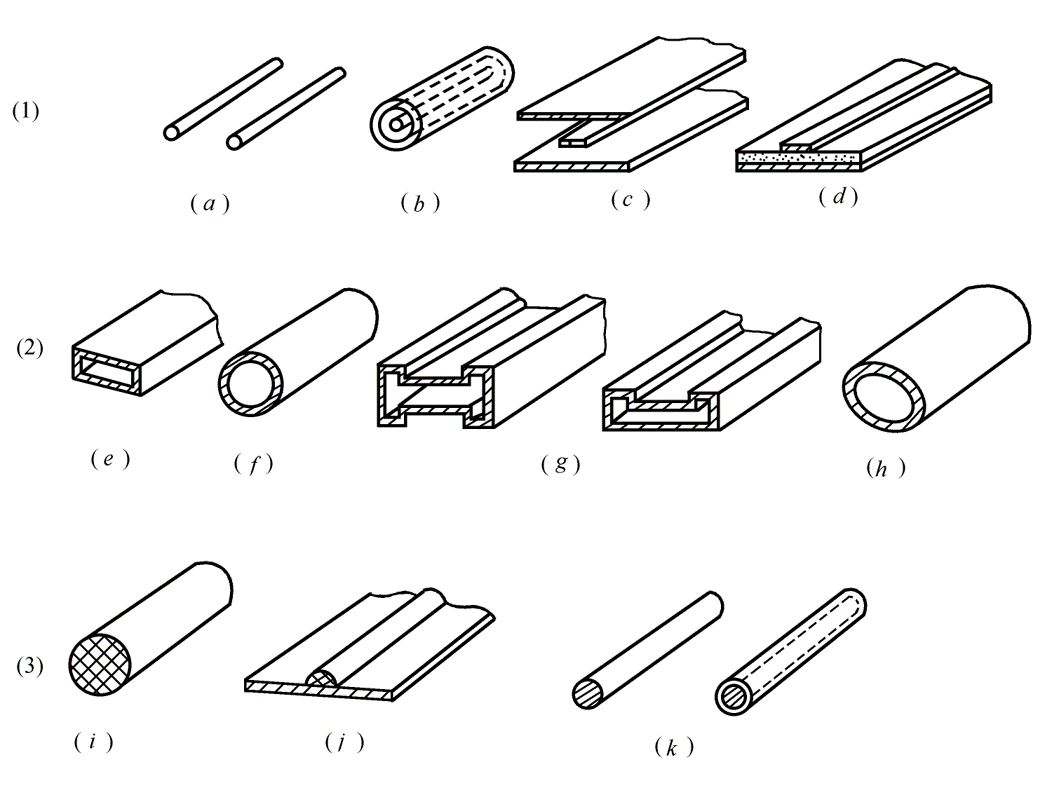
\includegraphics[width=9cm]{Cha3//guidesystem.png}
  \saveenum
\end{frame}

\subsection{长线理论与分布参数}
\begin{frame}{电路理论与传输线理论区别}
  电路理论与传输线理论之间的关键差别是\textbf{电尺寸}
  \begin{itemize}
    \item 低频电路 \Rightarrow 任意网络的尺寸比工作波长小得多,因而在电路中可以不考虑各点电压、电流的幅度和相位变化,沿线电压、电流只与时间因子有关,而与空间位置无关,分布参数产生的影响可以忽略
    \item 微波传输线 \Rightarrow 尺寸与工作波长可以比拟,或其长度是多个波长,这时传输线上电压、电流的幅值和相位不仅是时间的函数,还是位置的函数
  \end{itemize}
\end{frame}

\begin{frame}{分布参数效应}
  \begin{itemize}
    \item 分布参数效应
    \item 趋肤效应
  \end{itemize}
  \begin{tcolorbox}[colback=blue!0,colframe=blue!40!black,title=直流和微波频率下同一段圆导线电阻比较]
    微波频率下的电阻 $R_{MW}$ 由导线直径为 $D=1\mathrm{mm}$ 、厚度等于趋肤深度 $\delta_S$ 的空心导线的横截面部分决定,假设圆导体金属为铜,比较工作频率 $3\mathrm{GHz}$ 和直流工作情况下的电阻差异。
    $\mu=4\pi\times 10^{-7}\mathrm{H/m}, \sigma=5.8\times10^{7}\mathrm{S/m}$,由计算得知 $\delta_S=\dfrac{1}{\sqrt{\pi f\mu\sigma}}=1.2\mathrm{\mu m} $ \\
    $3\mathrm{GHz}$ 频率下的电阻 $R_{MW}=\dfrac{l}{\pi D\delta_S\sigma}$,直流工作电阻 $R_{DC}=\dfrac{l}{\pi (D^2/4)\sigma},\dfrac{R_{MW}}{R_{DC}}=\dfrac{D}{4\delta_S}=208$。$l$为该导线长度,
    假定其长度为 $5\mathrm{cm}$ ,则直流电阻仅为 $0.1\Omega/\mathrm{cm}$,但是在 $3\mathrm{GHz}$,其阻抗为 $20.8\Omega/\mathrm{cm}$,大出208倍。
  \end{tcolorbox}
\end{frame}

\begin{frame}{长线理论}
  \textbf{传输线}是以TEM导模的方式传送电磁波能量或信号的导行系统,其横向尺寸远小于其上工作波长。\\
  \textbf{传输线}有\textbf{长线}和\textbf{短线}之分。所谓长线是指传输线的几何长度与线上传输电磁波的波长比值(电长度)可相比拟,反之称为短线。\\
  \begin{align*}
    \text{长线}\Longrightarrow\text{分布参数电路} \\
    \text{短线}\Longrightarrow\text{集中参数电路} \\
    \text{分界线:}\widefbox{$l/\lambda\geq 0.1$}
  \end{align*}
  当频率提高到微波波段时,这些分布效应不可忽略,所以微波传输线是一种\textbf{分布参数电路}。这导致传输线上的电压和电流是随时间和空间位置而变化的二元函数。
\end{frame}

\begin{frame}{分布参数}
  \begin{itemize}
    \item 分布电阻:由于构成传输线导体的非理想产生;计算导体上的功率损耗
    \item 分布电导:由于传输线两导线间介质的非理想产生;计算介质中的功率损耗
    \item 分布电感:传输线的自感产生;存储在磁场中的能量
    \item 分布电容:两导线间存在电压降;存储在电场中的能量
  \end{itemize}
\end{frame}


\subsection{传输线的等效电路}
\begin{frame}{传输线的等效电路}
  根据传输线上的分布参数是否均匀分布,可将其分为均匀传输线和不均匀传输线。我们可以把均匀传输线分割成许多小的微元段$dz(dz<<\lambda)$,这样每个微元段可以看作集中参数电路,用一个$\Gamma$型网络来等效。于是整个传输线可等效成无穷多个$\Gamma$型网络的级联。\\
  \centering
  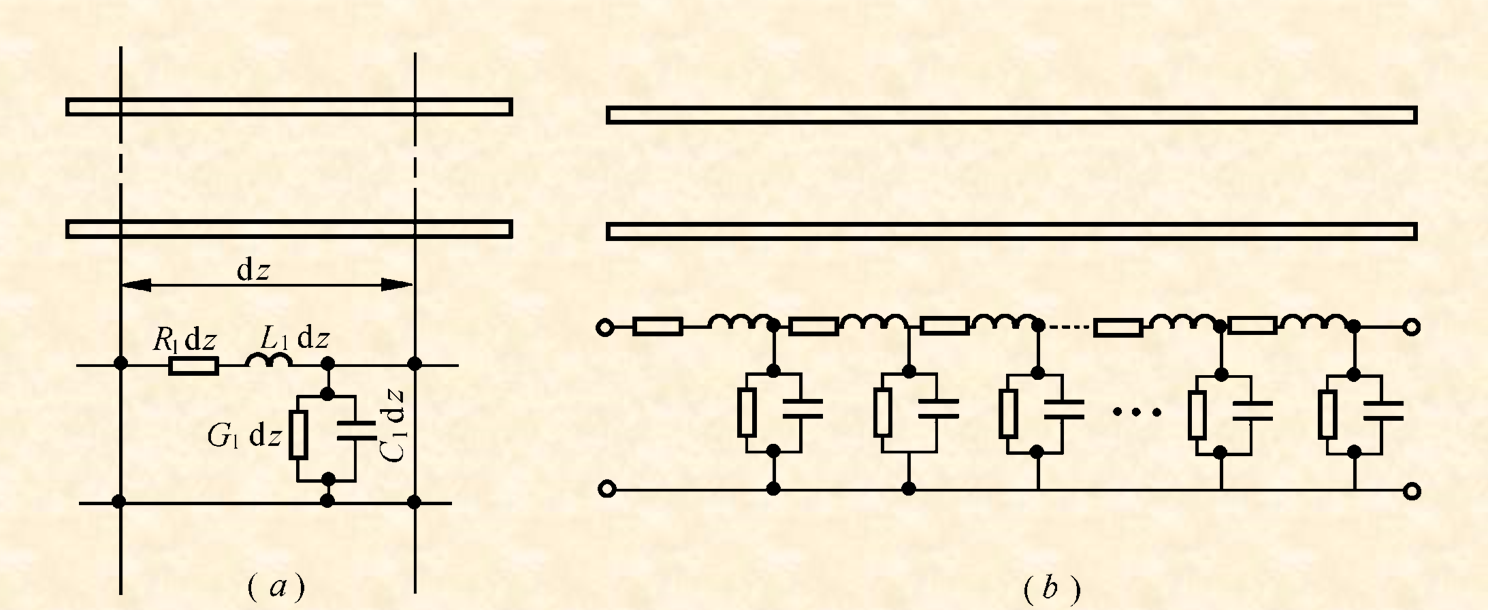
\includegraphics[width=9cm]{Cha3//transmissionline1.png}
\end{frame}


\begin{frame}{传输线的等效电路}
  双导线、同轴线和平行线传输线的分布参数\\
  \centering
  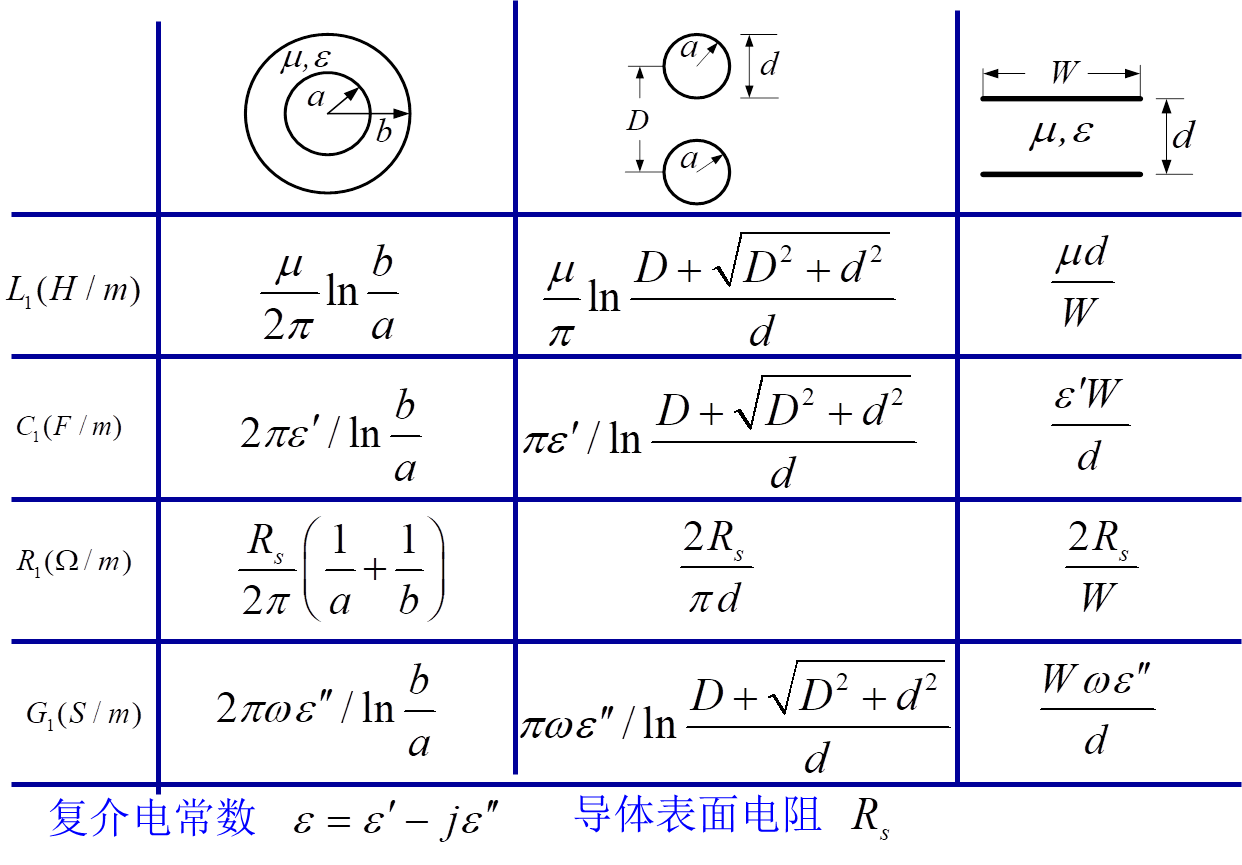
\includegraphics[width=9cm]{Cha3//tmlineparas.png}
\end{frame}

\subsection{电报方程及其求解}
\begin{frame}{电报方程}
  \begin{itemize}
    \item 一般传输线方程或电报方程\\
  \end{itemize}

  \centering
  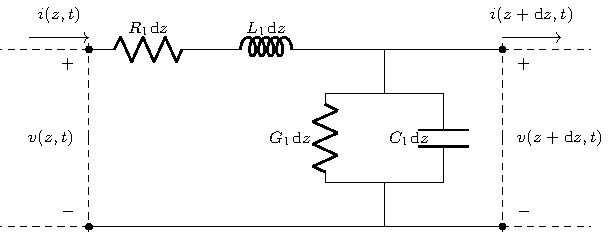
\includegraphics[width=8cm]{Cha3//circuit.pdf}

  \flushleft
  \fbox{$ v(z+\Delta z,t)=v(z,t)+\dfrac{\partial v(z,t)}{\partial z}\Delta z $}
  \flushright
  \fbox{$ i(z+\Delta z,t)=i(z,t)+\dfrac{\partial i(z,t)}{\partial z}\Delta z $}\\
  \begin{align*}
    \color{blue}{f(x)=f(x_{0})+f^{'}(x_{0})(x-x_{0})  +\frac{f^{''}(x_{0})}{2!}(x-x_{0})^{2}+\ldots} \\
    \color{blue}{+\frac{f^{n}(x_{0})}{n!}(x-x_{0})^{n}+R_{n}(x)}
  \end{align*}
\end{frame}

\begin{frame}{电报方程}
  \centering
  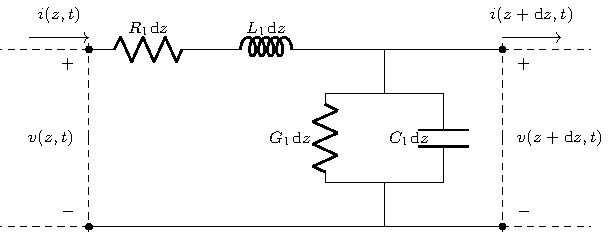
\includegraphics[width=8.5cm]{Cha3//circuit.pdf}
  \flushleft
  线元$\Delta z$上的电压、电流的变化为:
  \begin{empheq}[box=\widefbox]{align*}
    v(z,t)-v(z+\Delta z,t)=-\frac{\partial v(z,t)}{\partial z}\Delta z\\
    i(z,t)-i(z+\Delta z,t)=-\frac{\partial i(z,t)}{\partial z}\Delta z
  \end{empheq}
\end{frame}

\begin{frame}{电报方程}
  \centering
  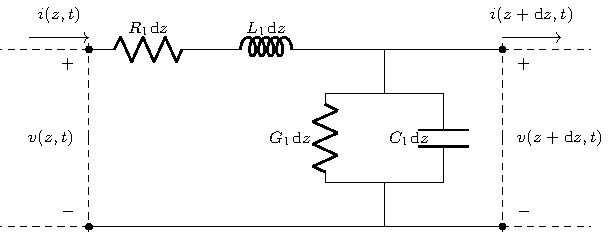
\includegraphics[width=8.5cm]{Cha3//circuit.pdf}
  \flushleft
  线元$\Delta z$上应用基尔霍夫定律,可得:
  \begin{empheq}[box=\widefbox]{align*}
    -\frac{\partial v(z,t)}{\partial z}\Delta z&=R_{1}\Delta z\cdot i(z,t)+L_{1}\Delta z\cdot\frac{\partial i(z,t)}{\partial t}\\
    -\frac{\partial i(z,t)}{\partial z}\Delta z&=G_{1}\Delta z\cdot v(z+\Delta z,t)+C_{1}\Delta z\cdot\frac{\partial v(z+\Delta z,t)}{\partial t}
  \end{empheq}
\end{frame}

\begin{frame}{电报方程}
  \begin{empheq}[box=\widefbox]{align*}
    -\frac{\partial v(z,t)}{\partial z}\Delta z&=R_{1}\Delta z\cdot i(z,t)+L_{1}\Delta z\cdot\frac{\partial i(z,t)}{\partial t}\\
    -\frac{\partial i(z,t)}{\partial z}\Delta z&=G_{1}\Delta z\cdot v(z+\Delta z,t)+C_{1}\Delta z\cdot\frac{\partial v(z+\Delta z,t)}{\partial t}
  \end{empheq}
  \flushleft
  令$\Delta z \rightarrow 0$
  \begin{empheq}[box=\widefbox]{align*}
    \frac{\partial v(z,t)}{\partial z}&=-R_{1}\cdot i(z,t)-L_{1}\cdot\frac{\partial i(z,t)}{\partial t}\\
    \frac{\partial i(z,t)}{\partial z}&=-G_{1}\cdot v(z,t)-C_{1}\cdot\frac{\partial v(z,t)}{\partial t}
  \end{empheq}
  \centering
  \textbf{一般传输线方程、电报方程}
\end{frame}

\begin{comment}
\newcommand{\mtikzmark}[1]{\tikz[overlay,remember picture]\node(#1){};}
\tikzset{mylabel/.style={align=center,fill=blue!10,font=\footnotesize}}
%\mytlabel[options]{start.mark}{end.mark}{text}

\newcommand\mytlabel[4][]{%
  \tikz[overlay,remember picture]
  {\draw[->]([yshift=-10pt]#2.north) -- node[mylabel,#1]{#4}([yshift=6pt]#3.north);}
}
\end{comment}

\begin{frame}{电报方程}
  \begin{itemize}
    \item 时谐均匀传输线方程
  \end{itemize}
  \begin{empheq}[box=\widefbox]{align*}
    \frac{\partial v(z,t)}{\partial z}=-R_{1}\cdot i(z,t)-L_{1}\cdot\frac{\partial i(z,t)}{\partial t}\\
    \frac{\partial i(z,t)}{\partial z}=-G_{1}\cdot v(z,t)-C_{1}\cdot\frac{\partial v(z,t)}{\partial t}
  \end{empheq}
  \begin{columns}
    \begin{column}{0.5\linewidth}
      \begin{empheq}[box=\widefbox]{align*}
        v(z,t)=\mathrm{Re}\left[V(z)\mathrm{e}^{\mathrm{j}\omega t}\right]\\
        i(z,t)=\mathrm{Re}\left[I(z)\mathrm{e}^{\mathrm{j}\omega t}\right]
      \end{empheq}
    \end{column}
    \begin{column}{0.5\linewidth}
      分布参数:$R_{1}$,$L_{1}$,$C_{1}$,$G_{1}$不随位置变化
    \end{column}
  \end{columns}
\end{frame}

\begin{frame}{电报方程}
  \begin{empheq}[box=\widefbox]{align*}
    \frac{\mathrm{d}V(z)}{\mathrm{d}z}=-(R_{1}+\mathrm{j}\omega L_{1})I(z)=-Z_{1}I(z)\\
    Z_{1}=R_{1}+\mathrm{j}\omega L_{1} \text{:单位长度串联阻抗}
  \end{empheq}
  \begin{empheq}[box=\widefbox]{align*}
    \frac{\mathrm{d}I(z)}{\mathrm{d}z}=-(G_{1}+\mathrm{j}\omega C_{1})V(z)=-Y_{1}V(z)\\
    Y_{1}=G_{1}+\mathrm{j}\omega C_{1} \text{:单位长度并联导纳}
  \end{empheq}
  对$z$再微商
  \begin{align*}
    \frac{\mathrm{d}^2}{\mathrm{d}z^2}\left\{
    \begin{aligned}
      V(z) \\I(z)
    \end{aligned}
    \right\}-\gamma^2
    \left\{\begin{aligned}
             V(z) \\I(z)
           \end{aligned}\right\}=0
  \end{align*}
  \textbf{电压传播常数}:\fbox{$\gamma=\sqrt{Z_{1}Y_{1}}=\sqrt{(R_{1}+\mathrm{j}\omega L_{1})(G_{1}+\mathrm{j}\omega C_{1})}$}
\end{frame}


\begin{frame}{电报方程的解}
  \begin{itemize}
    \item 时谐传输线方程电压、电流通解
  \end{itemize}
  电压:
  \begin{empheq}[box=\widefbox]{align*}
    \color{blue}{V(z)=A_{1}\mathrm{e}^{-\gamma z}+A_{2}\mathrm{e}^{\gamma z}}
  \end{empheq}
  电流:
  \begin{empheq}[box=\widefbox]{align*}
    I(z)=-\frac{1}{R_{1}+\mathrm{j}\omega L_{1}}\frac{\mathrm{d}V(z)}{\mathrm{d}z}=\frac{1}{Z_{0}}(A_{1}\mathrm{e}^{-\gamma z}-A_{2}\mathrm{e}^{\gamma z})
  \end{empheq}
  $$\gamma=\sqrt{Z_{1}Y_{1}}=\sqrt{(R_{1}+\mathrm{j}\omega L_{1})(G_{1}+\mathrm{j}\omega C_{1})}=\alpha+\mathrm{j}\beta$$
  \textbf{特性阻抗}:
  \begin{empheq}[box=\widefbox]{align*}
    Z_{0}=\sqrt{\frac{R_{1}+\mathrm{j}\omega L_{1}}{G_{1}+\mathrm{j}\omega C_{1}}}
  \end{empheq}
\end{frame}

\begin{frame}{电报方程的解}
  \begin{itemize}
    \item \textbf{传输线的特性参数}
          \begin{itemize}
            \item 特性阻抗
          \end{itemize}
          \begin{align*}
            Z_{0}=\sqrt{\frac{R_{1}+\mathrm{j}\omega L_{1}}{G_{1}+\mathrm{j}\omega C_{1}}}
          \end{align*}
          传输线上\textbf{行波}的电压与电流之比称为传输线的特性阻抗\\
          $$\text{无耗线}R_{1}=G_{1}=0\quad Z_{0}=\sqrt{\frac{L_{1}}{C_{1}}}$$\\
          微波低耗线$R_{1}<<\omega L_{1},G_{1}<<\omega C_{1}$\\
          $$Z_{0}=\sqrt{\frac{R_{1}+\mathrm{j}\omega L_{1}}{G_{1}+\mathrm{j}\omega C_{1}}}\approx\sqrt{\frac{L_{1}}{C_{1}}}\left[1+\frac{1}{2}\left(\frac{R_{1}}
              {\mathrm{j}\omega L_{1}}-\frac{G_{1}}{\mathrm{j}\omega C_{1}}\right)\right]$$
  \end{itemize}
\end{frame}

\begin{frame}{电报方程的解}
  \begin{itemize}
    \item \textbf{双导线特性阻抗}\\
          $$Z_{0}=120\ln\left[\frac{D}{d}+\sqrt{\left(\frac{D}{d}\right)^{2}-1}\right]$$
    \item \textbf{同轴线特性阻抗}\\
          $$Z_{0}=\frac{60}{\sqrt{\epsilon_{r}}}\ln\frac{b}{a}$$
    \item \textbf{平行板传输线特性阻抗}\\
          $$Z_{0}=\frac{d}{W}\eta$$
  \end{itemize}
\end{frame}

\begin{frame}{电报方程的解}
  \begin{itemize}
    \item \textbf{传播常数}
  \end{itemize}
  描述导行波沿着导行系统传播过程中的\textbf{衰减}和\textbf{相位}变化的参数
  \begin{empheq}[box=\widefbox]{align*}
    \gamma = \sqrt{(R_{1}+\mathrm{j}\omega L_{1})(G_{1}+\mathrm{j}\omega C_{1})}=\alpha+\mathrm{j}\beta
  \end{empheq}
  $\alpha$——衰减常数,单位$\mathrm{Np/m}$或$\mathrm{dB/m}$\quad $(1\mathrm{Np}=8.686\mathrm{dB})$\\
  $\beta$——相位常数,单位$\mathrm{rad/m}$\\
  \centering
  $\text{无耗线}\quad \alpha=0$\quad \fbox{$\beta=\omega\sqrt{L_{1}C_{1}}$}
\end{frame}

\begin{frame}{电报方程的解}
  微波低耗线\quad$R_{1}<<\omega L_{1},G_{1}<<\omega C_{1}$
  \begin{align*}
    \gamma & =\sqrt{(R_{1}+\mathrm{j}\omega L_{1})(G_{1}+\mathrm{j}\omega C_{1})}=\alpha+\mathrm{j}\beta                                                           \\
           & =\sqrt{(\mathrm{j}\omega)^{2}L_{1}C_{1}}\sqrt{\left(1+\frac{R_{1}}{\mathrm{j}\omega L_{1}}\right)\left(1+\frac{G_{1}}{\mathrm{j}\omega C_{1}}\right)} \\
           & \approx\frac{1}{2}\left(R_{1}\sqrt{C_{1}/L_{1}}+G_{1}\sqrt{L_{1}/C_{1}}\right)+\mathrm{j}\omega\sqrt{L_{1}C_{1}}
  \end{align*}
  \begin{columns}
    \begin{column}{0.65\linewidth}
      \begin{empheq}[box=\widefbox]{align*}
        \therefore\alpha=\frac{R_{1}}{2Z_{0}}+\frac{G_{1}Z_{0}}{2}=\alpha_{c}+\alpha_{d}
      \end{empheq}
      $\alpha_{c}$:分布电阻产生的导体衰减常数\\
      $\alpha_{d}$:漏电导产生的介质衰减常数
    \end{column}
    \begin{column}{0.35\linewidth}
      \begin{empheq}[box=\widefbox]{align*}
        \therefore\beta=\omega\sqrt{L_{1}C_{1}}
      \end{empheq}
      $\beta$:近似于无耗传输线的相位常数
    \end{column}
  \end{columns}
\end{frame}

\begin{frame}{电报方程的解}
  对于TEM导波:\\
  $$k_{c}=0,\lambda_{c}=\infty$$\\
  其相速度为\\
  $$v_{p}=v=\frac{\omega}{\beta}=\frac{1}{\sqrt{L_{1}C_{1}}}$$\\
  波长为\\
  $$\lambda_{g}=\lambda=\frac{2\pi}{\beta}=\frac{v_{p}}{f}$$\\
  特性阻抗为\\
  $$Z_{0}=\sqrt{\frac{L_{1}}{C_{1}}}=\frac{1}{v_{p}C_{1}}=v_{p}L_{1}$$\\
  \textbf{传输线的特性阻抗可由单位长度分布电容或分布电感求得}
\end{frame}

\begin{frame}{电报方程的解}
  \begin{itemize}
    \item 传输线方程的边界条件和解
  \end{itemize}
  \begin{columns}
    \begin{column}{0.35\linewidth}
      端接条件确定常数:\\
      终端条件\\
      始端条件\\
      信号源和负载条件
    \end{column}
    \begin{column}{0.65\linewidth}
      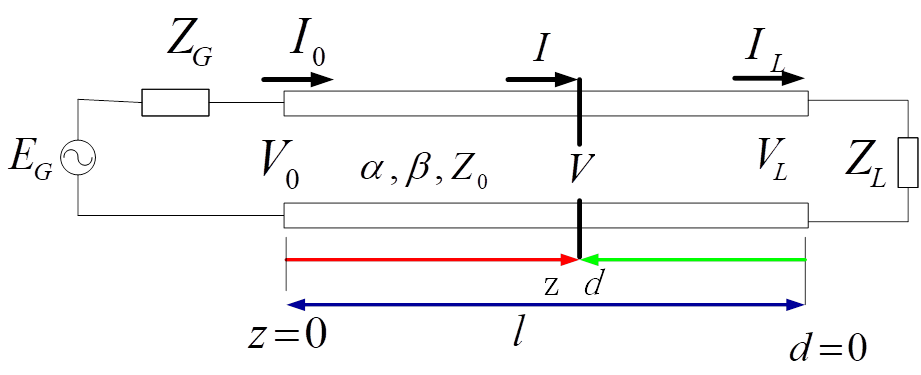
\includegraphics[width=7cm]{Cha3//tmlineboundary.png}
    \end{column}
  \end{columns}
  \textbf{终端条件}解:
  \begin{columns}
    \begin{column}{0.5\linewidth}
      \begin{empheq}[box=\widefbox]{align*}
        V(z)=A_{1}\mathrm{e}^{-\gamma z}+A_{2}\mathrm{e}^{\gamma z}
      \end{empheq}
    \end{column}
    \begin{column}{0.5\linewidth}
      \begin{empheq}[box=\widefbox]{align*}
        I(z)=(A_{1}\mathrm{e}^{-\gamma z}-A_{2}\mathrm{e}^{\gamma z})/Z_{0}
      \end{empheq}
    \end{column}
  \end{columns}
  \begin{empheq}[box=\widefbox]{align*}
    V(l)=V_{L}=A_{1}\mathrm{e}^{-\gamma l}+A_{2}\mathrm{e}^{\gamma l}\\
    I(l)=I_{L}=\frac{1}{Z_{0}}(A_{1}\mathrm{e}^{-\gamma l}-A_{2}\mathrm{e}^{\gamma l})
  \end{empheq}
\end{frame}


\begin{frame}{电报方程的解}
  \begin{empheq}[box=\widefbox]{align*}
    A_{1}=\frac{V_{L}+I_{L}Z_{0}}{2}\mathrm{e}^{\gamma l},A_{2}=\frac{V_{L}-I_{L}Z_{0}}{2}\mathrm{e}^{-\gamma l}
  \end{empheq}
  代入:
  \begin{columns}
    \begin{column}{0.45\linewidth}
      \begin{empheq}[box=\widefbox]{align*}
        V(z)=A_{1}\mathrm{e}^{-\gamma z}+A_{2}\mathrm{e}^{\gamma z}
      \end{empheq}
    \end{column}
    \begin{column}{0.45\linewidth}
      \begin{empheq}[box=\widefbox]{align*}
        I(z)=(A_{1}\mathrm{e}^{-\gamma z}-A_{2}\mathrm{e}^{\gamma z})/Z_{0}
      \end{empheq}
    \end{column}
  \end{columns}
  对于终端边界条件场合,我们常采用$d$(终端出发)坐标系$d$,换坐标\fbox{$d=l-z$}
  \begin{empheq}[box=\widefbox]{align*}
    V(d)=\frac{V_{L}+I_{L}Z_{0}}{2}\mathrm{e}^{\gamma d}+\frac{V_{L}-I_{L}Z_{0}}{2}\mathrm{e}^{-\gamma d}=V^{+}(d)+V^{-}(d)\\
    I(d)=\frac{V_{L}+I_{L}Z_{0}}{2Z_{0}}\mathrm{e}^{\gamma d}-\frac{V_{L}-I_{L}Z_{0}}{2Z_{0}}\mathrm{e}^{-\gamma d}=I^{+}(d)+I^{-}(d)
  \end{empheq}
\end{frame}

\begin{frame}{电报方程的解}
  \begin{empheq}[box=\widefbox]{align*}
    V(d)=\frac{V_{L}+I_{L}Z_{0}}{2}\mathrm{e}^{\gamma d}+\frac{V_{L}-I_{L}Z_{0}}{2}\mathrm{e}^{-\gamma d}=V^{+}(d)+V^{-}(d)\\
    I(d)=\frac{V_{L}+I_{L}Z_{0}}{2Z_{0}}\mathrm{e}^{\gamma d}-\frac{V_{L}-I_{L}Z_{0}}{2Z_{0}}\mathrm{e}^{-\gamma d}=I^{+}(d)+I^{-}(d)
  \end{empheq}
  \begin{empheq}[box=\widefbox]{align*}
    V(d)=\frac{\mathrm{e}^{\gamma d}+\mathrm{e}^{-\gamma d}}{2}V_{L}+\frac{\mathrm{e}^{\gamma d}-\mathrm{e}^{-\gamma d}}{2}Z_{0}I_{L}\\
    I(d)=\frac{\mathrm{e}^{\gamma d}-\mathrm{e}^{-\gamma d}}{2}\frac{1}{Z_{0}}V_{L}+\frac{\mathrm{e}^{\gamma d}+\mathrm{e}^{-\gamma d}}{2}I_{L}
  \end{empheq}
  \begin{align*}
    \begin{bmatrix}
      V(d) \\I(d)
    \end{bmatrix}
    =
    \begin{bmatrix}
      \cosh\gamma d           & Z_{0}\sinh\gamma d \\
      Z_{0}^{-1}\sinh\gamma d & \cosh\gamma d
    \end{bmatrix}
    \begin{bmatrix}
      V_{L} \\I_{L}
    \end{bmatrix}
  \end{align*}
\end{frame}


\begin{frame}{电报方程的解}
  \textbf{始端条件解}:已知始端电压和电流$V_{0},I_{0}$ \\
  \fbox{$V(z)=A_{1}\mathrm{e}^{-\gamma z}+A_{2}\mathrm{e}^{\gamma z}$}
  \fbox{$I(z)=(A_{1}\mathrm{e}^{-\gamma z}-A_{2}\mathrm{e}^{\gamma z})/Z_{0}$}\\
  \begin{columns}
    \begin{column}{0.3\linewidth}
      \begin{align*}
        V_{0}=A_{1}+A_{2} \\
        I_{0}=(A_{1}-A_{2})/Z_{0}
      \end{align*}
    \end{column}
    \begin{column}{0.1\linewidth}
      \centering
      $ \longrightarrow $
    \end{column}
    \begin{column}{0.6\linewidth}
      \begin{empheq}[box=\fbox]{align*}
        A_{1}=\frac{V_{0}+I_{0}Z_{0}}{2}\quad A_{2}=\frac{V_{0}-I_{0}Z_{0}}{2}
      \end{empheq}
    \end{column}
  \end{columns}
  \begin{empheq}[box=\widefbox]{align*}
    V(z)=\frac{V_{0}+I_{0}Z_{0}}{2}\mathrm{e}^{-\gamma z}+\frac{V_{0}-I_{0}Z_{0}}{2}\mathrm{e}^{\gamma z}\\
    I(z)=\frac{V_{0}+I_{0}Z_{0}}{2Z_{0}}\mathrm{e}^{-\gamma z}-\frac{V_{0}-I_{0}Z_{0}}{2Z_{0}}\mathrm{e}^{\gamma z}
  \end{empheq}
  \begin{align*}
    \begin{bmatrix}
      V(z) \\I(z)
    \end{bmatrix}
    =
    \begin{bmatrix}
      \cosh\gamma z            & -Z_{0}\sinh\gamma z \\
      -Z_{0}^{-1}\sinh\gamma z & \cosh\gamma z
    \end{bmatrix}
    \begin{bmatrix}
      V_{0} \\I_{0}
    \end{bmatrix}
  \end{align*}
\end{frame}

\begin{frame}{电报方程的解}
  \textbf{信号源和负载条件解}:
  已知信号源电动势 $E_{G}$、
  内阻抗 $Z_{G}$、
  负载阻抗 $Z_{L}$
  \begin{empheq}[box=\widefbox]{align*}
    V(d)=\frac{E_{G}Z_{0}}{Z_{G}+Z_{0}}\cdot\frac{\mathrm{e}^{-\gamma l}}{1-\Gamma_{L}\Gamma_{G}\mathrm{e}^{-2\gamma l}}(\mathrm{e}^{\gamma d}+\Gamma_{L}\mathrm{e}^{-\gamma d})\\
    I(d)=\frac{E_{G}}{Z_{G}+Z_{0}}\cdot\frac{\mathrm{e}^{-\gamma l}}{1-\Gamma_{L}\Gamma_{G}\mathrm{e}^{-2\gamma l}}(\mathrm{e}^{\gamma d}-\Gamma_{L}\mathrm{e}^{-\gamma d})
  \end{empheq}
  \begin{align*}
    \Gamma_{L}=\frac{Z_{L}-Z_{0}}{Z_{L}+Z_{0}}\quad \Gamma_{G}=\frac{Z_{G}-Z_{0}}{Z_{G}+Z_{0}}\quad\text{反射系数}
  \end{align*}
\end{frame}

\subsection{传输线特征参数}
\begin{frame}
  \begin{itemize}
    \item 微波阻抗——由微波传输线上的电压和电流决定的,是\textbf{分布参数}阻抗。(低频传输线阻抗是\textbf{集中参数}阻抗)
    \item 微波阻抗——与导行系统上导波的反射或者驻波特性密切相关,即与导行系统的状态或者特性密切相关。
    \item 微波阻抗不能直接测量,需要借助反射参量或者驻波参量的直接测量而间接获得。
  \end{itemize}
\end{frame}

\begin{frame}{传输线特征参数}
  \begin{enumerate}
    \item \textbf{分布参数阻抗}
          \saveenum
  \end{enumerate}
  \centering
  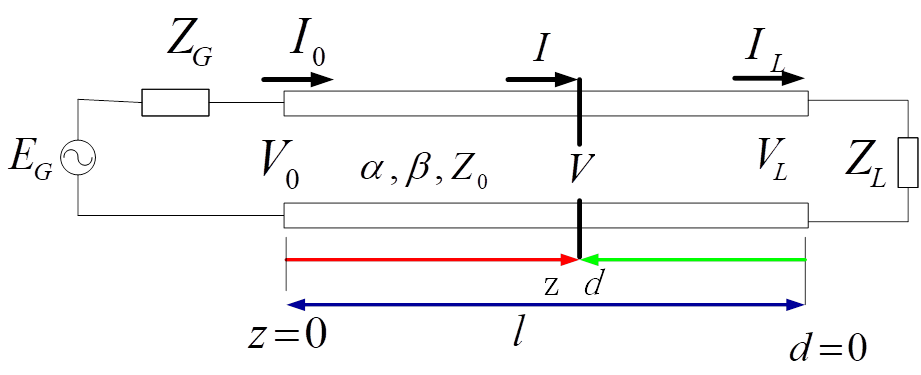
\includegraphics[width=8cm]{Cha3//tmlineboundary.png}
  \begin{align*}
    \begin{bmatrix}
      V(d) \\I(d)
    \end{bmatrix}=
    \begin{bmatrix}
      \cosh\gamma d\quad Z_{0}\sinh\gamma d \\
      Z_{0}^{-1}\sinh\gamma d\quad \cosh\gamma d
    \end{bmatrix}
    \begin{bmatrix}
      V_{L} \\I_{L}
    \end{bmatrix}
  \end{align*}
  \flushleft
  传输线终端接负载阻抗$Z_{L}$时,距离终端$d$处向负载方向看去的输入阻抗定义为该处的电压$V(z)$与电流$I(z)$之比,即
\end{frame}

\begin{frame}{传输线特征参数}
  \begin{empheq}[box=\widefbox]{align*}
    Z_{in}(d)=\frac{V_{L}\cosh\gamma d+I_{L}Z_{0}\sinh\gamma d}{I_{L}\cosh\gamma d+\frac{V_{L}\sin\beta d}{Z_{0}}}=Z_{0}\frac{Z_{L}+Z_{0}\tanh\gamma d}{Z_{0}+Z_{L}\tanh\gamma d}
  \end{empheq}
  \flushleft
  均匀无耗传输线\\
  $$\alpha=0,\gamma=\mathrm{j}\beta,\tanh\gamma d=\tanh(\mathrm{j}\beta d)=\mathrm{j}\tan\beta d$$
  \begin{columns}
    \begin{column}{0.4\linewidth}
      传输线的阻抗(从$d$点向负载看的输入阻抗,或视在阻抗)
    \end{column}
    \begin{column}{0.6\linewidth}
      \begin{empheq}[box=\widefbox]{align*}
        Z_{in}(d)=Z_{0}\frac{Z_{L}+\mathrm{j}Z_{0}\tan\beta d}{Z_{0}+\mathrm{j}Z_{L}\tan\beta d}
      \end{empheq}
    \end{column}
  \end{columns}
  \flushleft
  对给定的传输线和负载阻抗,线上各点的输入阻抗随至终端的距离$d$的不同而作周期(周期为$\lambda/2$)变化,是一种\textbf{分布参数阻抗}。它不能直接测量。
\end{frame}

\begin{frame}{传输线特征参数}
  \flushleft
  均匀无耗传输线\\
  \begin{empheq}[box=\widefbox]{align*}
    Z_{in}(d)=Z_{0}\frac{Z_{L}+\mathrm{j}Z_{0}\tan\beta d}{Z_{0}+\mathrm{j}Z_{L}\tan\beta d}
  \end{empheq}
  \begin{itemize}
    \item 传输线阻抗,随位置$d$而变,分布于沿线各点,且与负载有关,是一种分布参数阻抗(Distributed Impedance)。由于微波频率下,电压与电流缺乏明确的物理意义,不能直接测量,故传输线阻抗也不能直接测量。
    \item 传输线阻抗具有阻抗变换作用,$Z_{L}$通过线段$d$变换成$Z_{in}(d)$。
    \item 传输线阻抗呈现周期性变化。
  \end{itemize}
\end{frame}

\begin{frame}{传输线特征参数}
  \flushleft
  在一些特殊位置点上,有如下简单阻抗关系:
  \begin{empheq}[box=\widefbox]{align*}
    & Z_{in}(l)=Z_{L}\qquad l=n\frac{\lambda}{2}(n=0,1,2,\ldots)\\
    & Z_{in}(l)=\frac{Z_{0}^{2}}{Z_{L}}\qquad l=(2n+1)\frac{\lambda}{4}(n=0,1,2,\ldots)
  \end{empheq}
  \begin{itemize}
    \item 传输线上距负载为半波长整数倍的各点输入阻抗等于负载阻抗;\textbf{半波长的重复性}
    \item 距负载为四分之一波长奇数倍的各点输入阻抗等于特性阻抗的平方与负载阻抗的比值
    \item 当$Z_{0}$为实数,$Z_{L}$为复数负载时,四分之一波长的传输线具有变换阻抗性质的作用。\textbf{四分之一波长变换性}
  \end{itemize}
\end{frame}


\begin{frame}{传输线特征参数}
  \flushleft
  在许多情况下,例如并联电路的阻抗计算,采用导纳比较方便:
  \begin{empheq}[box=\widefbox]{align*}
    Y_{in}(d)=\frac{1}{Z_{in}(d)}=Y_{0}\frac{Y_{L}+\mathrm{j}Y_{0}\tan\beta d}{Y_{0}+\mathrm{j}Y_{L}\tan\beta d}
  \end{empheq}
\end{frame}

\begin{frame}{传输线特征参数}
  \begin{enumerate}
    \resume
    \item 反射参量
          \saveenum
  \end{enumerate}
  \begin{empheq}[box=\widefbox]{align*}
    V(d)=\frac{V_{L}+I_{L}Z_{0}}{2}\mathrm{e}^{\gamma d}+\frac{V_{L}-I_{L}Z_{0}}{2}\mathrm{e}^{-\gamma d}
  \end{empheq}
  \begin{itemize}
    \item 反射系数(Reflection Coefficient)
  \end{itemize}
  距终端$d$处的反射波电压$V^{-}(d)$与入射波电压$V^{+}(d)$之比定义为该处的\textbf{电压反射系数}$\Gamma_{v}(d)$,即
  \begin{align*}
    \Gamma_{v}(d) & =\frac{V^{-}(d)}{V^{+}(d)}=\frac{A_{2}\mathrm{e}^{-\gamma d}}{A_{1}\mathrm{e}^{\gamma d}}                                \\
                  & =\frac{V_{L}-I_{L}Z_{0}}{V_{L}+I_{L}Z_{0}}\mathrm{e}^{-2\gamma d}=\frac{Z_{L}-Z_{0}}{Z_{L}+Z_{0}}\mathrm{e}^{-2\gamma d}
  \end{align*}
\end{frame}

\begin{frame}{传输线特征参数}
  \begin{columns}
    \begin{column}{0.35\linewidth}
      电流反射系数
    \end{column}
    \begin{column}{0.65\linewidth}
      \begin{empheq}[box=\widefbox]{align*}
        I(d)=\frac{V_{L}+I_{L}Z_{0}}{2Z_{0}}\mathrm{e}^{\gamma d}-\frac{V_{L}-I_{L}Z_{0}}{2Z_{0}}\mathrm{e}^{-\gamma d}
      \end{empheq}
    \end{column}
  \end{columns}
  \begin{align*}
    \Gamma_{I}(d)=\frac{I^{-}(d)}{I^{+}(d)}=-\frac{A_{2}}{A_{1}}\mathrm{e}^{-2\gamma d}=-\Gamma_{V}(d)
  \end{align*}
  终端反射系数
  \begin{columns}
    \begin{column}{0.45\linewidth}
      \begin{align*}
         & \Gamma_{L}=\frac{A_{2}}{A_{1}}=\frac{Z_{L}-Z_{0}}{Z_{L}+Z_{0}}                                                                                 \\
         & =\left\lvert\frac{Z_{L}-Z_{0}}{Z_{L}+Z_{0}}\right\rvert \mathrm{e}^{\mathrm{j}\Phi_{L}}=\lvert\Gamma_{L}\rvert \mathrm{e}^{\mathrm{j}\Phi_{L}}
      \end{align*}
    \end{column}
    \begin{column}{0.45\linewidth}
      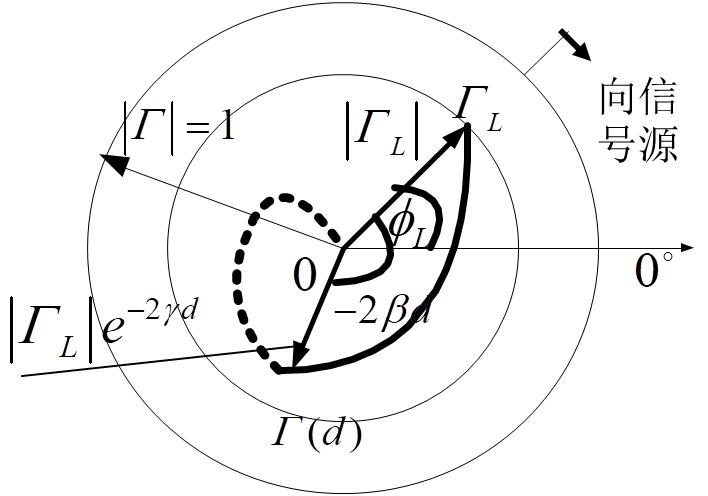
\includegraphics[width=4cm]{Cha3//chart1.png}
    \end{column}
  \end{columns}
  $$\Gamma(d)=\Gamma_{L}\mathrm{e}^{-2\gamma d}\text{传输线上任一点反射系数与终端反射系数的关系}$$
\end{frame}

\begin{frame}{传输线特征参数}
  无耗线情况
  \begin{empheq}[box=\widefbox]{align*}
    \Gamma(d)=\Gamma_{L}\mathrm{e}^{-\mathrm{j}2\beta d}=\lvert\Gamma_{L}\rvert \mathrm{e}^{\mathrm{j}(\Phi_{L}-2\beta d)}
  \end{empheq}
  \begin{columns}
    \begin{column}{0.5\linewidth}
      $\Gamma(d)$的大小和相位均在单位圆内,大小不变,相位以$-2\beta d$的角度沿等圆周向信号源(顺时针)方向变化。
    \end{column}
    \begin{column}{0.5\linewidth}
      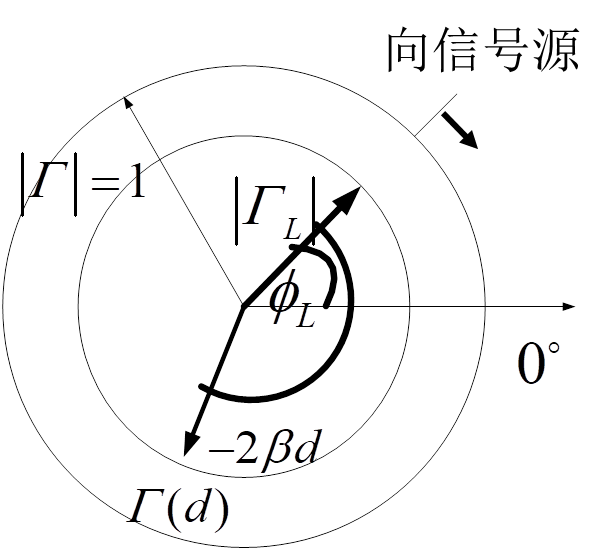
\includegraphics[width=4.5cm]{Cha3//chart2.png}
    \end{column}
  \end{columns}
\end{frame}

\begin{frame}{传输线特征参数}
  \begin{itemize}
    \item 阻抗与反射系数关系
  \end{itemize}
  \begin{align*}
     & V(d)=V^{+}(d)+V^{-}(d)=V^{+}(d)[1+\Gamma(d)] \\
     & I(d)=I^{+}(d)+I^{-}(d)=I^{+}(d)[1-\Gamma(d)]
  \end{align*}
  输入阻抗与反射系数间的关系
  \begin{empheq}[box=\widefbox]{align*}
    Z_{in}(d)=\frac{V^{+}(d)[1+\Gamma(d)]}{I^{+}(d)[1-\Gamma(d)]}=Z_{0}\frac{1+\Gamma(d)}{1-\Gamma(d)}
  \end{empheq}
\end{frame}

\begin{frame}{传输线特征参数}
  \begin{empheq}[box=\widefbox]{align*}
    Z_{in}(d)=\frac{V^{+}(d)[1+\Gamma(d)]}{I^{+}(d)[1-\Gamma(d)]}=Z_{0}\frac{1+\Gamma(d)}{1-\Gamma(d)}
  \end{empheq}
  当传输线特性阻抗$Z_{0}$一定时,传输线上任意一点$d$处的阻抗$Z_{in}(d)$与该点的反射系数$\Gamma(d)$一一对应。可以通过测量反射系数获得传输线输入阻抗。\\
  \textbf{归一化}阻抗
  \begin{empheq}[box=\widefbox]{align*}
    z_{in}(d)=\frac{Z_{in}(d)}{Z_{0}}=\frac{1+\Gamma(d)}{1-\Gamma(d)}
  \end{empheq}
\end{frame}

\begin{frame}{传输线特征参数}
  \begin{itemize}
    \item 传输系数$T$\qquad 描述传输线上的功率传输关系
  \end{itemize}
  \begin{columns}
    \begin{column}{0.5\linewidth}
      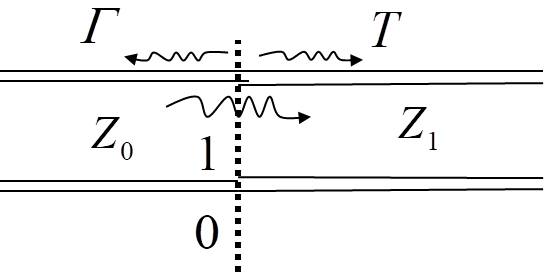
\includegraphics[width=4cm]{Cha3//transPara.png}
    \end{column}
    \begin{column}{0.5\linewidth}
      \begin{align*}
        T=\frac{\text{传输电压或电流}}{\text{入射电压或电流}}=\frac{V^{t}}{V^{+}}=\frac{I^{t}}{I^{+}}
      \end{align*}
    \end{column}
  \end{columns}
  \begin{empheq}[box=\fbox]{align*}
    & V(z)=V^{+}_{0}(\mathrm{e}^{-\mathrm{j}\beta z}+\Gamma \mathrm{e}^{\mathrm{j}\beta z})\quad z<0\\
    & V(z)=V_{0}^{+}T\mathrm{e}^{-\mathrm{j}\beta z}\qquad\qquad\quad z>0
  \end{empheq}
  $Z=0$处两电压连续
  \begin{empheq}[box=\widefbox]{align*}
    T=1+\Gamma=1+\frac{Z_{1}-Z_{0}}{Z_{1}+Z_{0}}=\frac{2Z_{1}}{Z_{1}+Z_{0}}
  \end{empheq}
  插入损耗
  \begin{empheq}[box=\widefbox]{align*}
    L_{T}=-20\lg\lvert T \rvert \qquad (dB)
  \end{empheq}
\end{frame}

%\begin{comment}
\begin{frame}{传输线特征参数}
  \begin{enumerate}
    \resume
    \item \textbf{驻波参量}
          \saveenum
  \end{enumerate}
  \begin{itemize}
    \item 电压驻波比(VSWR)与行波系数K\\
          传输线上各点的电压和电流一般由入射波和反射波叠加而成,其结果在线上形成驻波,沿线各点的电压和电流的振幅不同,以$\lambda/2$周期变化。\\
          波腹点——振幅最大点\\
          波谷点——振幅最小点\qquad 波节点——振幅等于零的点\\
          \textbf{电压(或电流)驻波比VSWR}:定义为传输线上电压(或电流)振幅的最大值与最小值之比,或电压驻波系数$\rho$
          \begin{empheq}[box=\widefbox]{align*}
            VSWR=\rho=\frac{\lvert V\rvert_{max}}{\lvert V\rvert_{min}}=\frac{\lvert I\rvert_{max}}{\lvert I\rvert_{min}}
          \end{empheq}
  \end{itemize}
\end{frame}

\begin{frame}{传输线特征参数}
  \textbf{行波系数K}:定义为传输线上电压(或电流)的最小值与最大值之比,故行波系数与驻波比互为倒数。
  \begin{empheq}[box=\widefbox]{align*}
    K=\frac{1}{VSWR}=\frac{\lvert V\rvert_{min}}{\lvert V\rvert_{max}}=\frac{\lvert I\rvert_{min}}{\lvert I\rvert_{max}}
  \end{empheq}
\end{frame}

\begin{frame}{传输线特征参数}
  传输线任意点电压和电流
  \begin{align*}
    V(d)=V^{+}(d)[1+\lvert\Gamma_{L}\rvert \mathrm{e}^{\mathrm{j}(\Phi_{L}-2\beta d)}] \\
    I(d)=I^{+}(d)[1-\lvert\Gamma_{L}\rvert \mathrm{e}^{\mathrm{j}(\Phi_{L}-2\beta d)}]
  \end{align*}
  \begin{columns}
    \begin{column}{0.5\linewidth}
      当传输线上入射波与反射波同相叠加时,合成波出现最大值;而反向叠加时出现最小值。
    \end{column}
    \begin{column}{0.5\linewidth}
      \begin{align*}
        \lvert V(d)\rvert_{max}=v^{+}(d)[1+\lvert\Gamma_{L}\rvert] \\
        \lvert V(d)\rvert_{min}=v^{+}(d)[1-\lvert\Gamma_{L}\rvert]
      \end{align*}
    \end{column}
  \end{columns}
  驻波比与反射系数的关系式为:
  \begin{columns}
    \begin{column}{0.65\linewidth}
      \begin{empheq}[box=\widefbox]{align*}
        \rho=VSWR=\frac{\lvert V\rvert_{max}}{\lvert V\rvert_{min}}=\frac{1+\lvert\Gamma_{L}\rvert}{1-\lvert\Gamma_{L}\rvert}
      \end{empheq}
    \end{column}
    \begin{column}{0.35\linewidth}
      \begin{empheq}[box=\widefbox]{align*}
        \lvert\Gamma_{L}\rvert=\frac{\rho-1}{\rho+1}
      \end{empheq}
    \end{column}
  \end{columns}
\end{frame}
%\end{comment}

\begin{frame}{传输线特征参数}{沿线阻抗分布}
  线上任一点处的输入阻抗为:
  \begin{align*}
    Z_{in}(z)=Z_{0}\frac{Z_{L}+\mathrm{j}Z_{0}\tan\beta z}{Z_{0}+\mathrm{j}Z_{L}\tan\beta z}=R_{in}(z)+\mathrm{j}X_{in}(z)
  \end{align*}
  (1)阻抗的数值周期性变化,在电压的波腹点和波谷点,阻抗分别为最大值和最小值
  \begin{align*}
    Z_{in}(波腹)=\frac{\lvert U\rvert_{max}}{\lvert I\rvert_{min}}=Z_{0}\frac{1+\lvert\Gamma\rvert}{1-\lvert\Gamma\rvert}=Z_{0}\rho\qquad \text{开路} \\
    Z_{in}(波谷)=\frac{\lvert U\rvert_{min}}{\lvert I\rvert_{max}}=Z_{0}\frac{1-\lvert\Gamma\rvert}{1+\lvert\Gamma\rvert}=Z_{0}/\rho\qquad \text{短路}
  \end{align*}
  (2)每隔$\lambda/4$,阻抗性质变换一次;每隔$\lambda/2$,阻抗值重复一次。
\end{frame}

\begin{frame}{传输线特征参数}
  \begin{itemize}
    \item 阻抗与驻波参量的关系
  \end{itemize}
  由分布参数阻抗
  \begin{empheq}[box=\widefbox]{align*}
    Z_{in}(d)=Z_{0}\frac{Z_{L}+\mathrm{j}Z_{0}\tan\beta d}{Z_{0}+\mathrm{j}Z_{L}\tan\beta d}
  \end{empheq}
  \centering
  $\downarrow$
  \begin{empheq}[box=\widefbox]{align*}
    Z_{L}=Z_{0}\frac{Z_{in}(d)-\mathrm{j}Z_{0}\tan\beta d}{Z_{0}-\mathrm{j}Z_{in}(d)\tan\beta d}
  \end{empheq}
  \begin{columns}
    \begin{column}{0.6\linewidth}
      选取驻波最小点为测量点——距离负载的第一个电压驻波最小点位置
    \end{column}
    \begin{column}{0.4\linewidth}
      \begin{align*}
        Z_{in}(d_{min})=Z_{0}/VSWR=Z_{0}/\rho
      \end{align*}
    \end{column}
  \end{columns}
  \flushleft
  终端短路,确定电压波节点作参考点,接上负载测量参考点附近电压驻波最小点。
  \begin{columns}
    \begin{column}{0.5\linewidth}
      \begin{empheq}[box=\fbox]{align*}
        Z_{L}=Z_{0}\frac{1-\mathrm{j}\rho\tan\beta d_{min}}{\rho-\mathrm{j}\tan\beta d_{min}}
      \end{empheq}
    \end{column}
    \begin{column}{0.5\linewidth}
      负载阻抗和驻波参量一一对应
    \end{column}
  \end{columns}
\end{frame}

\begin{frame}{传输线特征参数}
  \begin{enumerate}
    \resume
    \item 传输功率
  \end{enumerate}
  均匀无耗传输线上任一点 $z$ 处的电压和电流可表示为
  \begin{align*}
    \begin{cases}
      V(z)=V_0^+\left[\mathrm{e}^{-\mathrm{j}\beta z}+\Gamma_L\mathrm{e}^{+\mathrm{j}\beta z} \right] \\
      I(z)=\dfrac{V_0^+}{Z_0}\left[ \mathrm{e}^{-\mathrm{j}\beta z}-\Gamma_L\mathrm{e}^{+\mathrm{j}\beta z}\right]
    \end{cases}
  \end{align*}
  则传输功率的一般表达式为:
  \begin{align*}
    P(z) & =\frac{1}{2}\mathrm{Re}\left\{V(z)I^*(z)\right\}=\frac{1}{2}\frac{|V_0^+|^2}{Z_0}\mathrm{Re}\left\{1-\Gamma_L^*\mathrm{e}^{-\mathrm{j}2\beta z}+\Gamma_L\mathrm{e}^{\mathrm{j}2\beta z}-|\Gamma_L|^2\right\} \\
         & =\frac{1}{2}\frac{|V_0^+|^2}{Z_0}(1-|\Gamma_L|^2)
  \end{align*}
  上式第一项为入射功率:$P^+(z)=\dfrac{1}{2}\dfrac{|V_0^+|^2}{Z_0}$,第二项为反射功率:$P^-(z)=\dfrac{1}{2}\dfrac{|V_0^+|^2}{Z_0}|\Gamma_L|^2$;所以,传输功率等于入射功率减去反射功率。
\end{frame}

\subsection{传输线工作状态}
\begin{frame}{传输线工作状态}
  任何传输线上的电压函数只可能是入射波和反射波的迭加(构成Standing Wave)。不同传输线的区别仅仅在于入射波和反射波的成分不同。换句话说,通解是完备的,我们不需要再找,也不可能再找到其他解。\\
  边界条件确定$A_{1}$和$A_{2}$。边界条件的求取过程中,也孕育着一种思想,即网络思想(Network Idea):已知输入求输出;或已知输出求输入。
\end{frame}

\begin{frame}{无耗传输线工作状态}
  \begin{empheq}[box=\widefbox]{align*}
    V(z)=A_{1}\mathrm{e}^{-\mathrm{j}\beta z}+A_{2}\mathrm{e}^{+\mathrm{j}\beta z}
  \end{empheq}
  \begin{empheq}[box=\widefbox]{align*}
    V(d) & =\frac{1}{2}(V_{L}+Z_{0}I_{L})\mathrm{e}^{\mathrm{j}\beta d}+\frac{1}{2}(V_{L}-Z_{0}I_{L})\mathrm{e}^{-\mathrm{j}\beta d}\\
    & =V^{+}(d)+V^{-}(d)
  \end{empheq}
  \begin{empheq}[box=\widefbox]{align*}
    I(z)=\frac{1}{Z_{0}}(A_{1}\mathrm{e}^{-\mathrm{j}\beta z}-A_{2}\mathrm{e}^{+\mathrm{j}\beta z})
  \end{empheq}
  \begin{empheq}[box=\widefbox]{align*}
    I(d) & =\frac{1}{2Z_{0}}(V_{L}+Z_{0}I_{L})\mathrm{e}^{\mathrm{j}\beta d}-\frac{1}{2Z_{0}}(V_{L}-Z_{0}I_{L})\mathrm{e}^{-\mathrm{j}\beta d}\\
    & =I^{+}(d)+I^{-}(d)
  \end{empheq}
\end{frame}


\begin{frame}{无耗传输线工作状态}
  \begin{itemize}
    \item 传输线上反射波的大小,可用反射系数的模、驻波比和行波系数三个参量来描述。\\
          \begin{columns}
            \begin{column}{0.5\linewidth}
              反射系数模的变化范围为\\
              驻波比的变化范围为\\
              行波系数的变化范围为
            \end{column}
            \begin{column}{0.3\linewidth}
              \fbox{$0\leq\lvert\Gamma\rvert\leq 1$}\\
              \fbox{$1\leq\rho\leq\infty$}\\
              \fbox{$0\leq K\leq 1$}
            \end{column}
          \end{columns}
    \item 传输线的工作状态一般分为三种:\\
          (1)行波状态 \qquad $\lvert\Gamma\rvert=0,\rho=1,K=1$ \\
          (2)行驻波状态\quad $0<\lvert\Gamma\rvert<1 \quad 1<\rho<\infty \quad 0<K<1$\\
          (3)驻波状态 \qquad $\lvert\Gamma\rvert=1 \quad \rho=\infty \quad K=0$
  \end{itemize}
\end{frame}

\begin{frame}{无耗传输线工作状态}
  \begin{enumerate}
    \item \textbf{行波状态(无反射情况)}
          \begin{columns}
            \begin{column}{0.4\linewidth}
              条件:\\
              $Z_{L}=Z_{0}\rightarrow$\\
              $\Gamma_{L}=0,\rho=1,K=1$
            \end{column}
            \begin{column}{0.6\linewidth}
              \begin{empheq}[box=\widefbox]{align*}
                \Gamma_{L}=\frac{A_{2}}{A_{1}}=\frac{Z_{L}-Z_{0}}{Z_{L}+Z_{0}}\\
                =\left\lvert\frac{Z_{L}-Z_{0}}{Z_{L}+Z_{0}}\right\rvert \mathrm{e}^{\mathrm{j}\Phi_{L}}=\lvert\Gamma_{L}\rvert \mathrm{e}^{\mathrm{j}\Phi_{L}}
              \end{empheq}
            \end{column}
          \end{columns}
          由始端条件解
          \begin{empheq}[box=\widefbox]{align*}
            V(z)=\frac{V_{0}+I_{0}Z_{0}}{2}\mathrm{e}^{-\mathrm{j}\beta z}=V_{0}^{+}\mathrm{e}^{-\mathrm{j}\beta z}\\
            I(z)=\frac{V_{0}+I_{0}Z_{0}}{2Z_{0}}\mathrm{e}^{-\mathrm{j}\beta z}=I_{0}^{+}\mathrm{e}^{-\mathrm{j}\beta z}
          \end{empheq}
          \saveenum
  \end{enumerate}
\end{frame}


\begin{frame}{无耗传输线工作状态}
  \begin{columns}
    \begin{column}{0.5\linewidth}
      \begin{empheq}[box=\widefbox]{align*}
        v(z,t)=\lvert V_{0}^{+}\rvert\cos(\omega t-\phi_{0}-\beta z)\\
        i(z,t)=\lvert I_{0}^{+}\rvert\cos(\omega t-\phi_{0}-\beta z)
      \end{empheq}
      $\phi_{0}$为初相角,行波状态下的分布规律:\\
      (1)线上电压和电流的振幅恒定不变\\
      (2)电压行波与电流行波同相,它们的相位是位置$z$和时间$t$的函数,$v(z,t)$和$i(z,t)$初相均为$\phi_{0}$,因为$Z_{0}$是实数\\
      (3)线上的输入阻抗处处相等,且均等于特性阻抗
    \end{column}
    \begin{column}{0.5\linewidth}
      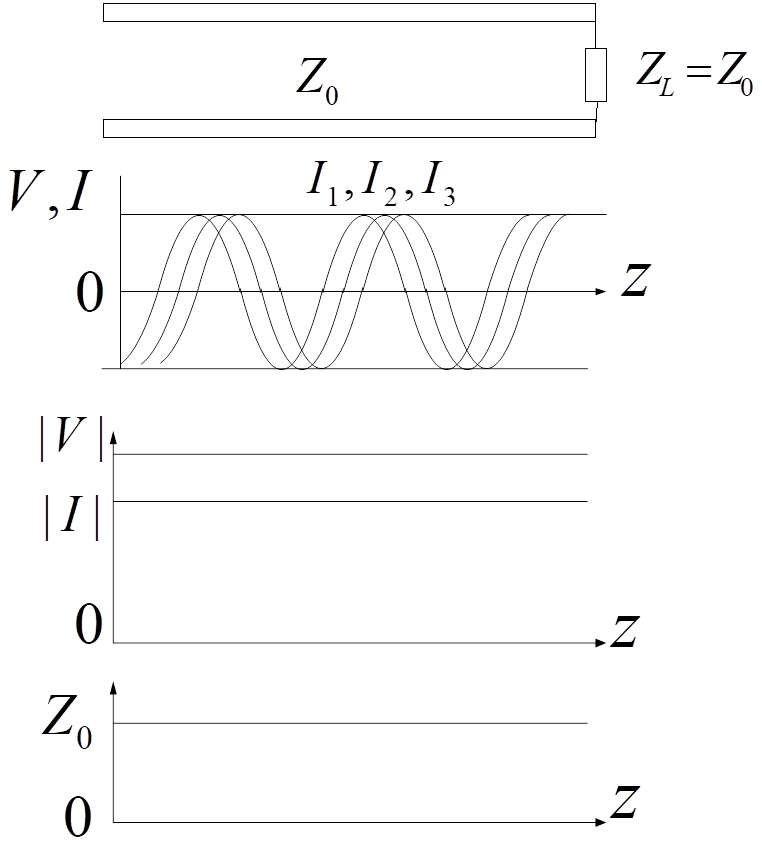
\includegraphics[width=5cm]{Cha3//xingbo.png}
    \end{column}
  \end{columns}
\end{frame}

\begin{frame}{无耗传输线工作状态}
  \begin{enumerate}
    \resume
    \item \textbf{驻波状态(全反射情况)}
          \saveenum
  \end{enumerate}
  反射系数模等于1的全反射情况称为驻波状态。
  \begin{empheq}[box=\widefbox]{align*}
    \Gamma_{L}=\frac{A_{2}}{A_{1}}=\frac{Z_{L}-Z_{0}}{Z_{L}+Z_{0}}=\left\lvert\frac{Z_{L}-Z_{0}}{Z_{L}+Z_{0}}\right\rvert \mathrm{e}^{\mathrm{j}\phi_{L}}=\lvert\Gamma_{L}\rvert \mathrm{e}^{\mathrm{j}\phi_{L}}
  \end{empheq}
  条件:终端短路;终端开路;终端接纯电抗负载\\
  \qquad \quad$Z_{L}=0$,\qquad$Z_{L}=\infty$,\qquad$Z_{L}=\pm \mathrm{j}X_{L}$\\
  终端的入射波将被全反射,沿线入射波与反射波迭加形成驻波分布。驻波状态意味着入射波功率一点也没有被负载吸收,即\textbf{负载与传输线完全失配}。
\end{frame}


\begin{frame}{无耗传输线工作状态}
  \begin{itemize}
    \item 终端短路
  \end{itemize}
  \begin{empheq}[box=\widefbox]{align*}
    Z_{L}=0,\Gamma_{L}=\frac{Z_{L}-Z_{0}}{Z_{L}+Z_{0}}=-1\rightarrow VSWR=\frac{1+\lvert\Gamma_{L}\rvert}{1-\lvert\Gamma_{L}\rvert}=\infty
  \end{empheq}
  \begin{align*}
    V(d) & =V^{+}(d)+V^{-}(d)=V_{L}^{+}(\mathrm{e}^{\mathrm{j}\beta d}-\mathrm{e}^{-\mathrm{j}\beta d})=\mathrm{j}2V_{L}^{+}\sin\beta d \\
    I(d) & =I^{+}(d)+I^{-}(d)=I_{L}^{+}(\mathrm{e}^{\mathrm{j}\beta d}+\mathrm{e}^{-\mathrm{j}\beta d})=2I_{L}^{+}\cos\beta d           \\
         & =\frac{2V_{L}^{+}}{Z_{0}}\cos\beta d
  \end{align*}
  短路时的驻波状态分布规律:\\
  (1)瞬时电压或电流在传输线的某个固定位置上随时间$t$作正弦或余弦变化,而在某一时刻随位置$d(z)$也作正弦或余弦变化,但瞬时电压和电流的时间相位差和空间相位差均为$\pi/2$,这表明传输线上没有功率传输。
\end{frame}

\begin{frame}{无耗传输线工作状态}
  \only<1>{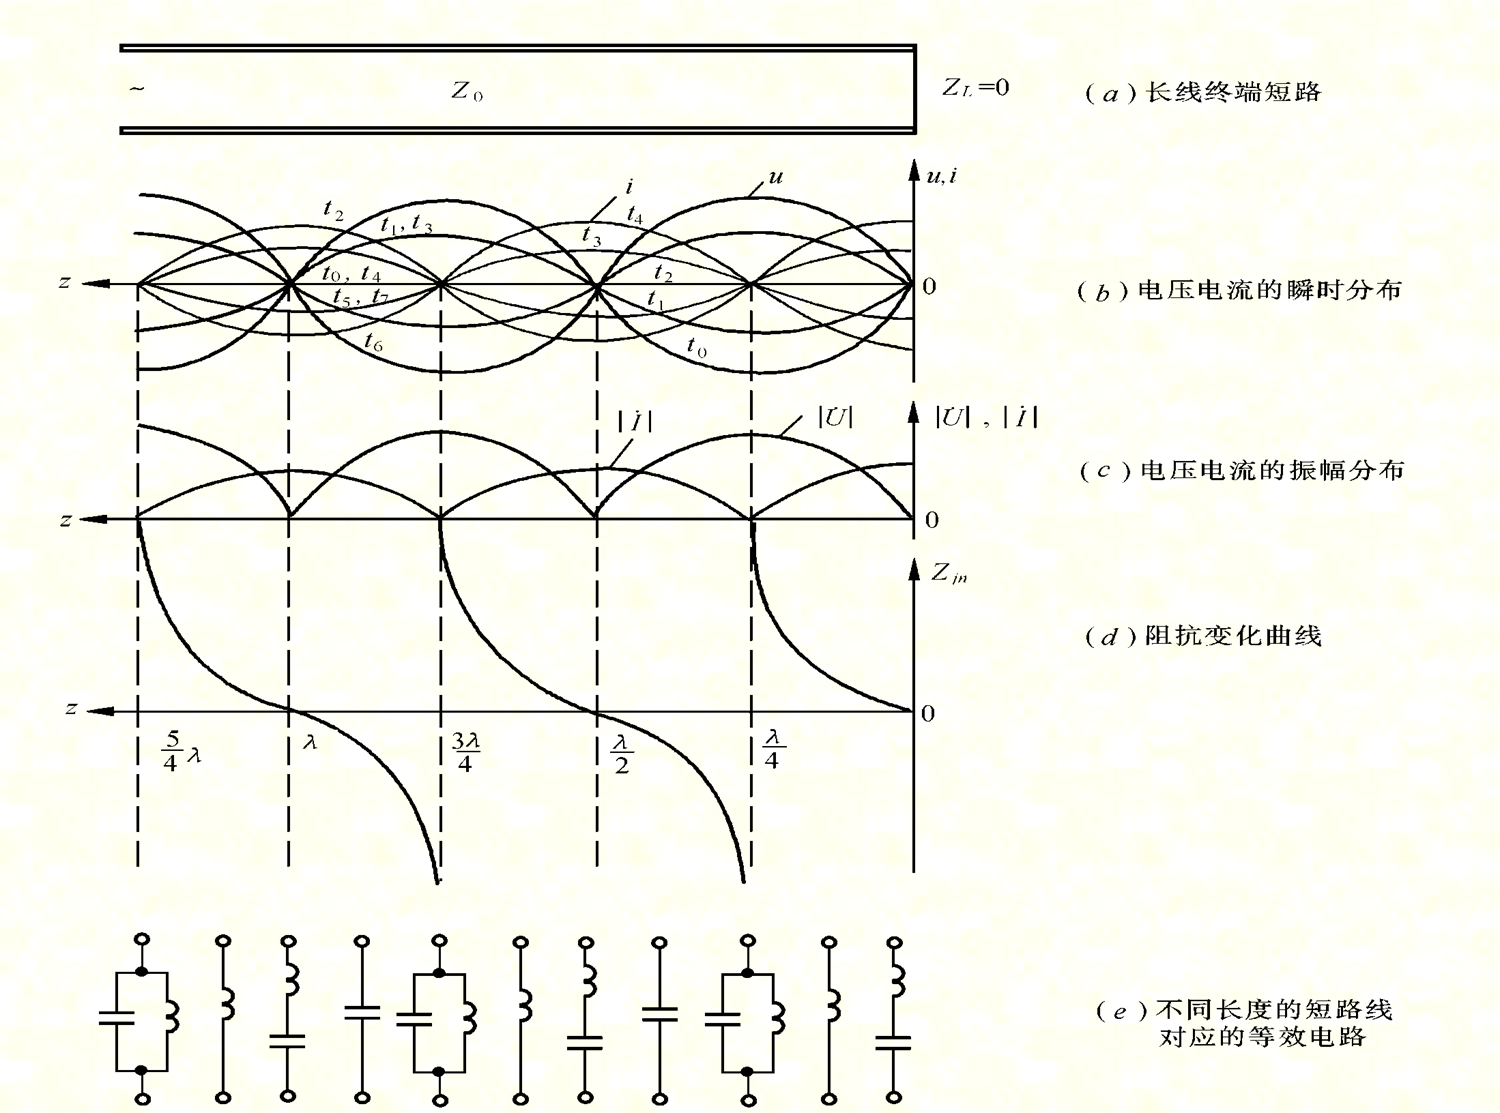
\includegraphics[width=10cm]{Cha3//duanlu.png}}
  \only<2>{\begin{columns}
      \begin{column}{0.55\linewidth}
        \begin{empheq}[box=\widefbox]{align*}
          d=(2n+1)\lambda/4,(n=0,1,\ldots)\\
          \lvert V\rvert_{max}=2\lvert V_{L}^{+}\rvert
        \end{empheq}
        \begin{empheq}[box=\widefbox]{align*}
          d=n\lambda/2,(n=0,1,\ldots)\\
          \lvert V\rvert_{min}=0
        \end{empheq}
      \end{column}
      \begin{column}{0.45\linewidth}
        (2)电压振幅最大值,而电流振幅恒为零,这些点称之为电压的波腹点和电流的波节点;\\
        电流振幅恒为最大值,而电压振幅恒为零,这些点称之为电流的波腹点和电压的波节点。
      \end{column}
    \end{columns}}
  \only<3>{
    \begin{table}[h!]
      \begin{center}
        \caption{终端短路情况}
        \begin{tabular}{|c|c|}
          \hline
          $ \beta d=n\pi $                                       & $ \beta d=(2n+1)\pi/2 $                                \\
          $ d=n\lambda/2 $                                       & $ d=(2n+1)\lambda/4 $                                  \\
          \hline
          $\text{电压节点}\lvert V(d)\rvert=0$                       & $\text{电压腹点}\lvert V(d)\rvert=2\lvert V_{L}^{+}\rvert$ \\
          $\text{电流腹点}\lvert I(d)\rvert=2\lvert I_{L}^{+}\rvert$ & $ \text{电流节点}\lvert I(d)\rvert=0$                      \\
          \hline
        \end{tabular}
      \end{center}
    \end{table}
  }
  \only<4>{(3)传输线终端短路时,输入阻抗为纯电抗。\\
    \begin{empheq}[box=\widefbox]{align*}
      Z_{in}^{sc}(d)=Z_{0}\frac{Z_{L}+\mathrm{j}Z_{0}\tan\beta d}{Z_{0}+\mathrm{j}Z_{L}\tan\beta d}=\mathrm{j}Z_{0}\tan\beta d=\mathrm{j}Z_{0}\tan\frac{2\pi d}{\lambda}=\mathrm{j}X_{in}
    \end{empheq}}
\end{frame}


\begin{frame}{无耗传输线工作状态}
  \begin{itemize}
    \item 终端开路
  \end{itemize}
  \begin{empheq}[box=\widefbox]{align*}
    Z_{L}=\infty,\Gamma_{L}=\frac{Z_{L}-Z_{0}}{Z_{L}+Z_{0}}=1\rightarrow VSWR=\frac{1+\lvert\Gamma_{L}\rvert}{1-\lvert\Gamma_{L}\rvert}=\infty
  \end{empheq}
  \begin{align*}
     & \Gamma_{L}=V_{L}^{-}/V_{L}^{+}=1 \quad V_{L}^{-}=V_{L}^{+} \\
     & V(d)=V^{+}(d)+V^{-}(d)=2V_{L}^{+}\cos\beta d               \\
     & I(d)=I^{+}(d)+I^{-}(d)=\mathrm{j}2I_{L}^{+}\sin\beta d     \\
     & Z_{in}^{oc}(d)=-\mathrm{j}Z_{0}\cot\beta d
  \end{align*}
  \begin{itemize}
    \item 终端短路
  \end{itemize}
  \begin{columns}
    \begin{column}{0.5\linewidth}

      \begin{empheq}[box=\widefbox]{align*}
        Z_{L}=0,\Gamma_{L}=-1\rightarrow VSWR=\infty
      \end{empheq}
    \end{column}
    \begin{column}{0.5\linewidth}
      \begin{empheq}[box=\widefbox]{align*}
        & V(d)=\mathrm{j}2V_{L}^{+}\sin\beta d\\
        & I(d)=2I_{L}^{+}\cos\beta d\\
        & Z_{in}^{sc}(d)=\mathrm{j}Z_{0}\tan\beta d
      \end{empheq}
    \end{column}
  \end{columns}
\end{frame}

\begin{frame}{无耗传输线工作状态}
  (1)负载处,或\fbox{$d=n\lambda/2,(n=0,1,\ldots)$}\\
  电流$I_{L}=0$为电流波节点,\\
  电压为最大值$V_{L}=2V_{L}^{+}$为电压波腹点
  \begin{table}[h!]
    \begin{center}
      \caption{终端开路情况}
      \begin{tabular}{|c|c|}
        \hline
        $\beta d=n\pi$                                  & $\beta d=(2n+1)\pi/2$                           \\
        $d=n\lambda/2$                                  & $d=(2n+1)\lambda/4$                             \\
        \hline
        电压腹点$\lvert V(d)\rvert=2\lvert V_{L}^{+}\rvert$ & 电压节点$\lvert V(d)=0\rvert$                       \\
        电流节点$\lvert I(d)=0\rvert$                       & 电流腹点$\lvert I(d)\rvert=2\lvert I_{L}^{+}\rvert$ \\
        \hline
      \end{tabular}
    \end{center}
  \end{table}
  (2)输入阻抗\\
  $Z_{in}^{oc}(d)=-\mathrm{j}Z_{0}\cot\beta d\Longleftrightarrow$ 短路 \fbox{$Z_{in}^{sc}=\mathrm{j}Z_{0}\tan\beta d$}\\
  经过观察:\textbf{把开路线可以看成是短路线移动$\lambda/4$而成}
\end{frame}


\begin{frame}{无耗传输线工作状态}
  \begin{columns}
    \begin{column}{0.5\linewidth}
      短路状态
      \begin{empheq}[box=\widefbox]{align*}
        & V(d)=\mathrm{j}2V_{L}^{+}\sin\beta d\\
        & I(d)=2I_{L}^{+}\cos\beta d
      \end{empheq}
      \begin{empheq}[box=\widefbox]{align*}
        Z(d)=\mathrm{j}Z_{0}\tan\beta d
      \end{empheq}
      作$d'=d+\lambda/4,V_{L}^{+}=\mathrm{j}\tilde V_{L}^{+}$变换,即可由开路线转化为短路线。不能疏忽了$V_{L}^{+}=\mathrm{j}\tilde V_{L}^{+}$的条件,长度$d'$移动条件只对$\lvert V_{L}^{+}\rvert$和阻抗有效,\textbf{相位}是不等价的。
    \end{column}
    \begin{column}{0.5\linewidth}
      开路状态
      \begin{empheq}[box=\widefbox]{align*}
        & V(d)=2V_{L}^{+}\cos\beta d\\
        & I(d)=\mathrm{j}2I_{L}^{+}\sin\beta d
      \end{empheq}
      \centering
      $\Downarrow$
      \begin{empheq}[box=\widefbox]{align*}
        & V(d')=\mathrm{j}2\tilde V_{L}^{+}\sin\beta d'\\
        & I(d')=2\tilde I_{L}^{+}\cos\beta d'
      \end{empheq}
      \begin{empheq}[box=\widefbox]{align*}
        Z(d)=-\mathrm{j}Z_{0}\cot\beta d
      \end{empheq}
      $\Downarrow$
      \begin{empheq}[box=\widefbox]{align*}
        Z(d')=\mathrm{j}Z_{0}\tan\beta d'
      \end{empheq}
    \end{column}
  \end{columns}
\end{frame}

\begin{frame}{无耗传输线工作状态}
  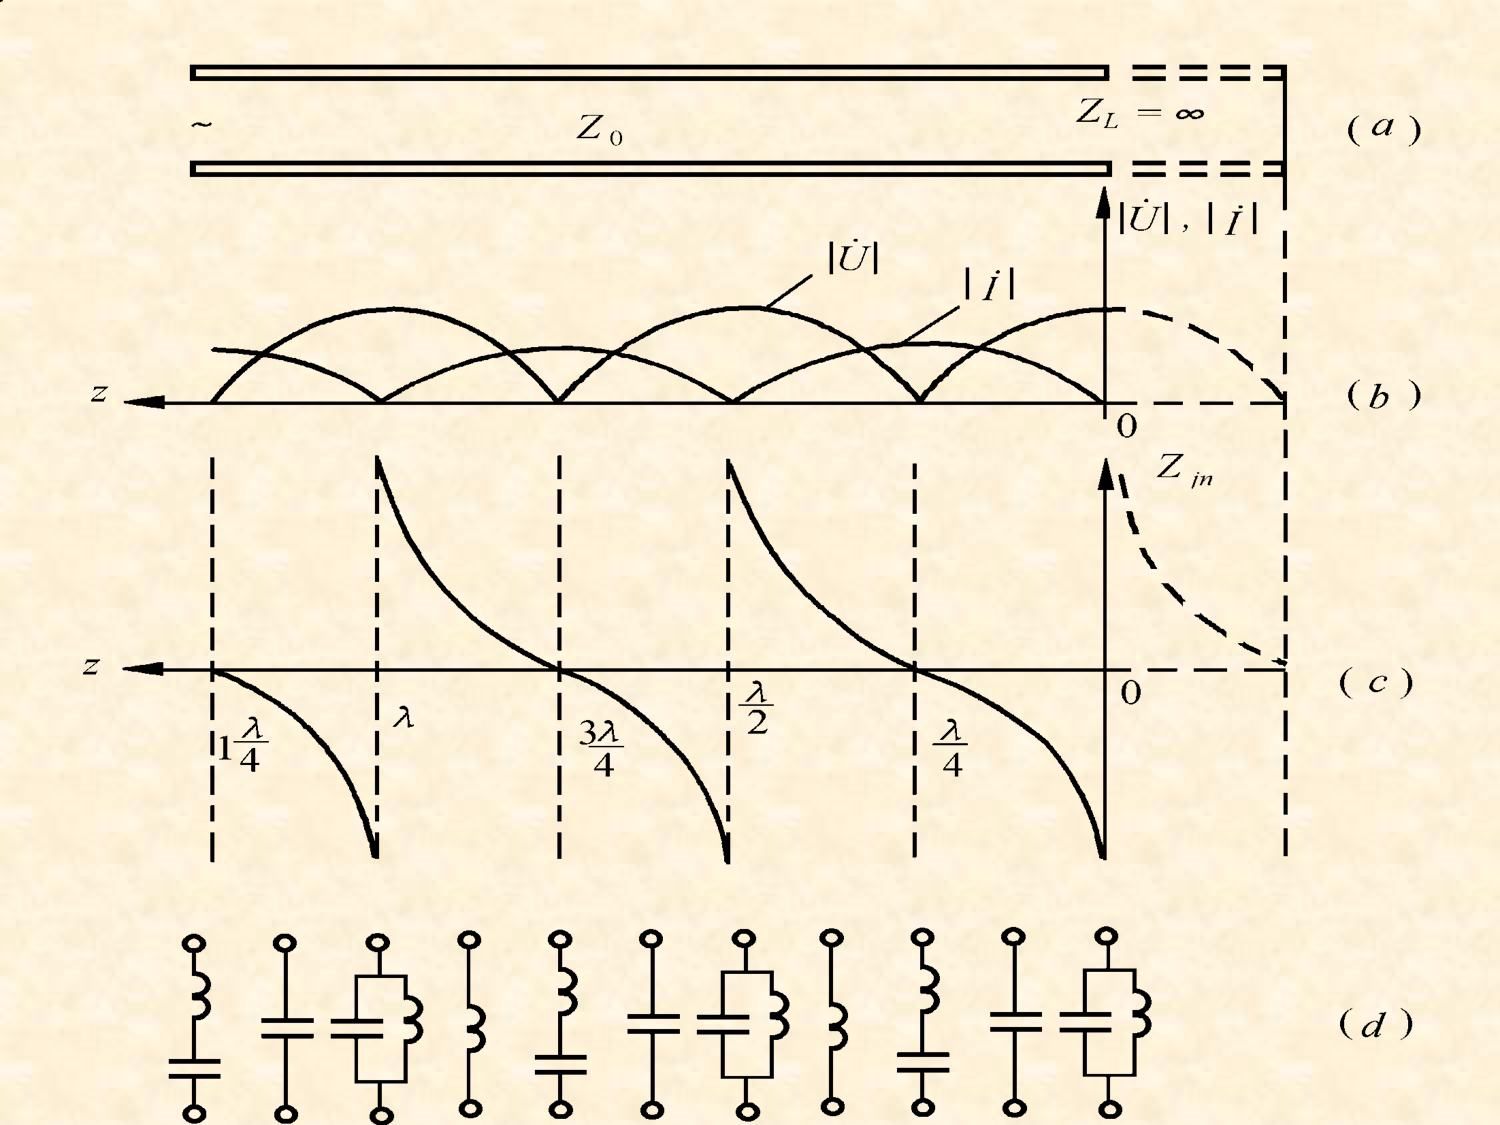
\includegraphics[width=10cm]{Cha3//kailu.png}
\end{frame}

\begin{frame}{无耗传输线工作状态}
  \begin{align*}
    Z_{in}^{oc}(d)=-\mathrm{j}Z_{0}\cot\beta d \qquad Z_{in}^{sc}(d)=\mathrm{j}Z_{0}\tan\beta d \\
    Z_{in}^{oc}(d)\cdot Z_{in}^{sc}(d)=Z_{0}^{2}
  \end{align*}
  \begin{itemize}
    \item 对于一定长度$d$的传输线,通过开路和短路的测量,可以得到如下参数:
  \end{itemize}
  \begin{align*}
     & Z_{0}=\sqrt{Z_{in}^{oc}(d)\cdot Z_{in}^{sc}(d)}                      \\
     & \beta=\frac{1}{d}\arctan\sqrt{\frac{Z_{in}^{sc}(d)}{Z_{in}^{oc}(d)}}
  \end{align*}
\end{frame}


\begin{frame}{无耗传输线工作状态}
  \begin{itemize}
    \item 终端接\textbf{纯电感}负载无耗线\quad \fbox{$Z_{L}=+\mathrm{j}X_{L}$}
  \end{itemize}
  \begin{align*}
    \Gamma_{L} & =\frac{Z_{L}-Z_{0}}{Z_{L}+Z_{0}}=\frac{\mathrm{j}X_{L}-Z_{0}}{\mathrm{j}X_{L}+Z_{0}}=\frac{(\mathrm{j}X_{L}-Z_{0})^2}{(\mathrm{j}X_{L}+Z_{0})(\mathrm{j}X_{L}-Z_{0})} \\
               & =\frac{Z_{0}^{2}-X_{L}^{2}-2\mathrm{j}Z_{0}X_{L}}{Z_{0}^{2}+X_{L}^{2}}=\lvert\Gamma_{L}\rvert \mathrm{e}^{\mathrm{j}\phi_{L}}
  \end{align*}
  \begin{align*}
    \therefore\lvert\Gamma_{L}\rvert=\frac{\sqrt{(Z_{0}^{2}-X_{L}^{2})^2+4Z_{0}^{2}X_{L}^{2}}}{Z_{0}^{2}+X_{L}^{2}}=\frac{\sqrt{(Z_{0}^{2}+X_{L}^{2})^2}}{Z_{0}^{2}+X_{L}^{2}}=1
  \end{align*}
  \begin{empheq}[box=\widefbox]{align*}
    \phi_{L}=\arctan\frac{2X_LZ_0}{X_L^2-Z_0^2}
  \end{empheq}
  终端产生全反射,形成驻波,但终端既不是电压波腹点也不是波节点
\end{frame}

\begin{frame}{无耗传输线工作状态}
  \begin{columns}
    \begin{column}{0.55\linewidth}
      可见此时终端也产生全反射,线上形成驻波;但此时终端$(d=0)$既不是电压波节点也不是电压波腹点。沿线的电压、电流和阻抗分布曲线可将电感负载用一段小于$\lambda/4$的短路线来等效后获得。
    \end{column}
    \begin{column}{0.45\linewidth}
      
\includegraphics[width=4.5cm]{Cha3//diangan1.png}
      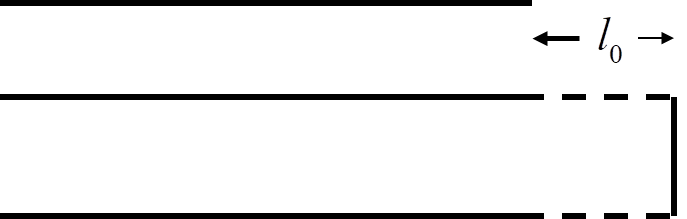
\includegraphics[width=4.5cm]{Cha3//diangan2.png}
    \end{column}
  \end{columns}
  \begin{columns}
    \begin{column}{0.55\linewidth}
      短路线输入阻抗:
      \begin{empheq}[box=\widefbox]{align*}
        Z_{in}^{sc}(d)=\mathrm{j}Z_{0}\tan\beta d=\mathrm{j}X_{L}
      \end{empheq}
      故有等效短路线长度:
      \begin{empheq}[box=\widefbox]{align*}
        l_{es}& =\frac{1}{\beta}\tan^{-1}\left(\frac{X_L}{Z_0}\right)\\
        & =\frac{\lambda}{2\pi}\arctan\left(\frac{X_L}{Z_0}\right)
      \end{empheq}
    \end{column}
    \begin{column}{0.45\linewidth}
      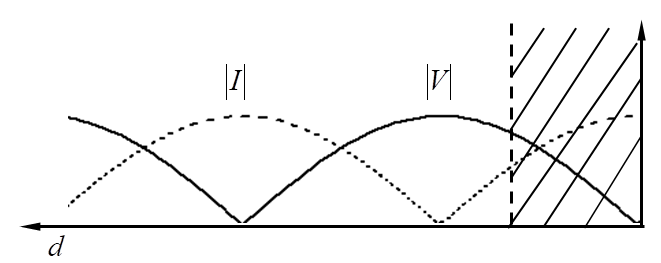
\includegraphics[width=4.5cm]{Cha3//diangan3.png}
      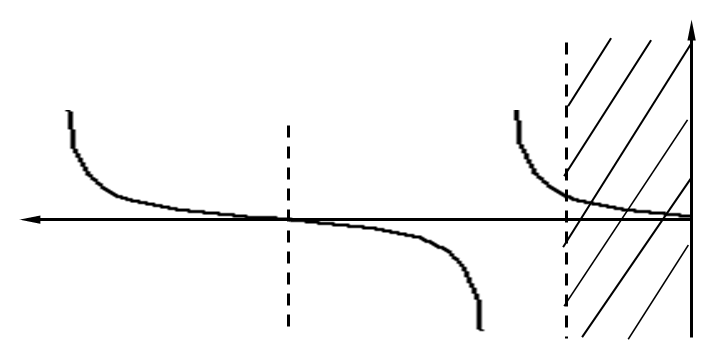
\includegraphics[width=4.5cm]{Cha3//diangan4.png}
    \end{column}
  \end{columns}
\end{frame}


\begin{frame}{无耗传输线工作状态}
  \begin{itemize}
    \item 终端接\textbf{纯电容}负载无耗线\quad \fbox{$Z_L=-\mathrm{j}X_L$}
  \end{itemize}
  \begin{align*}
    \Gamma_L=\frac{Z_L-Z_0}{Z_L+Z_0}=\frac{\mathrm{j}X_L+Z_0}{\mathrm{j}X_L-Z_0}=\lvert\Gamma_L\rvert \mathrm{e}^{-\mathrm{j}\phi_L} \\
    \lvert\Gamma_L\rvert=1 \qquad \phi_L=\arctan\frac{-2X_{L}Z_{0}}{X_{L}^{2}-Z_{0}^{2}}
  \end{align*}
  可见此时终端也产生全反射,线上形成驻波;但此时终端$(d=0)$既不是电压波节点也不是电压波腹点。沿线的电压、电流和阻抗分布曲线可将电容负载用一段小于$\lambda/4$的开路线来等效后获得。
  \begin{align*}
    Z_{in}^{oc}(d)=-\mathrm{j}Z_0\cot\beta d=-\mathrm{j}X_L
  \end{align*}
  \begin{empheq}[box=\widefbox]{align*}
    l_{eo} =\frac{1}{\beta}\cot^{-1}\left(\frac{X_L}{Z_0}\right)=\frac{\lambda}{2\pi}\cot^{-1}\left(\frac{X_L}{Z_0}\right)
  \end{empheq}
\end{frame}

\begin{frame}{无耗传输线工作状态}
  \centering
  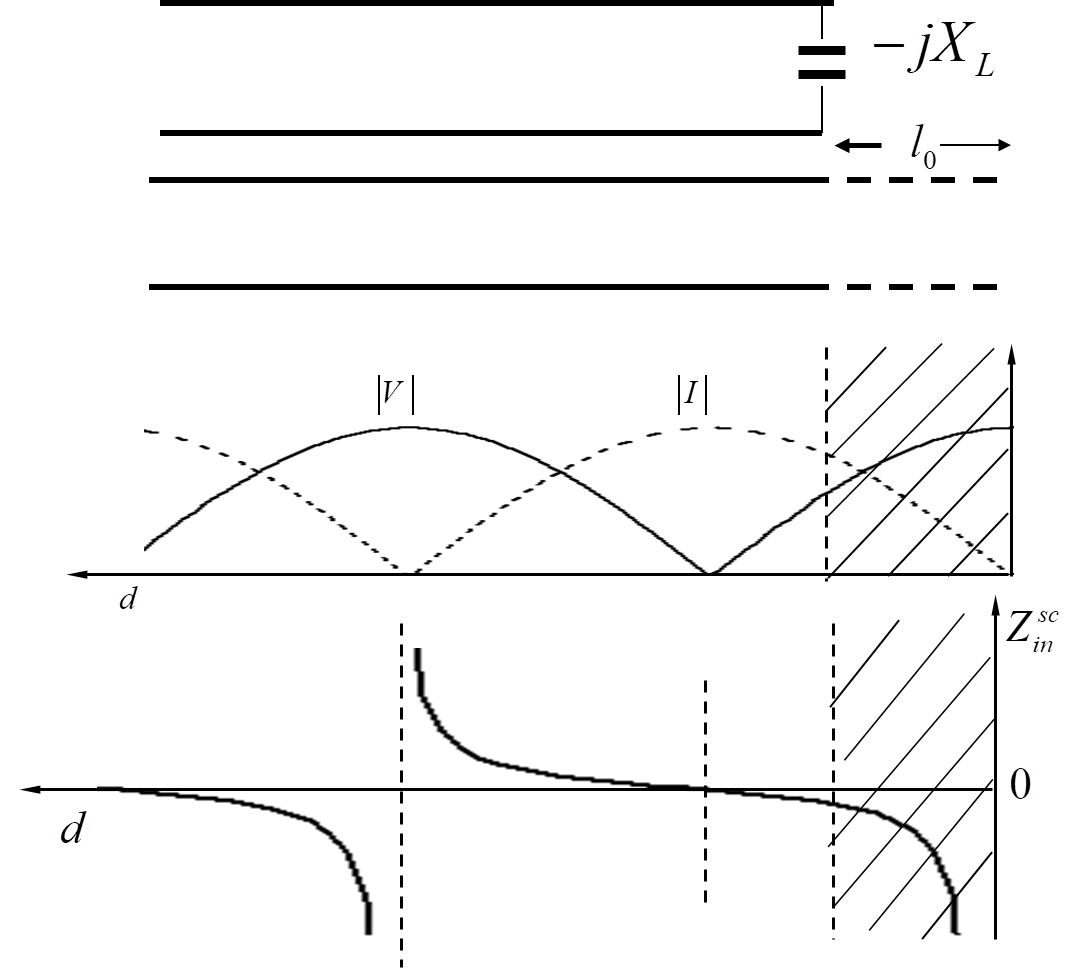
\includegraphics[width=8.5cm]{Cha3//dianrong.png}
\end{frame}


\begin{frame}{无耗传输线工作状态}
  阻抗的一般公式\quad \fbox{$Z_L=\mathrm{j}X_L$}
  \begin{align*}
    Z_{in}(d) & =Z_{0}\frac{Z_L+\mathrm{j}Z_0\tan\beta d}{Z_0+\mathrm{j}Z_L\tan\beta d}                                                                     \\
              & =\mathrm{j}Z_0\frac{X_L+Z_0\tan\beta d}{Z_0-X_L\tan\beta d}=\mathrm{j}Z_0\frac{\dfrac{X_L}{Z_0}+\tan\beta d}{1-\dfrac{X_L}{Z_0}\tan\beta d}
  \end{align*}
  此电抗也可用一段特性阻抗为$Z_0$、长度为$l_0$的短路线等效,长度$l_0$可由下式确定\\
  假设:$$\frac{X_L}{Z_0}=\tan\beta l_0 \qquad Z_{in}(d)=\mathrm{j}Z_0\tan\beta(d+l_0)$$
  \begin{align*}
    l_0=\frac{\lambda}{2\pi}\arctan\frac{X_L}{Z_0}\quad \Longrightarrow \quad
    \left\{
    \begin{aligned}
      l_0>0 \quad X_L\text{为感性} \\
      l_0<0 \quad X_L\text{为容性}
    \end{aligned}
    \right.
  \end{align*}
\end{frame}


\begin{frame}{无耗传输线工作状态}
  \begin{empheq}[box=\widefbox]{align*}
    X_L=Z_0\tan\frac{2\pi}{\lambda}l_0\quad \Longrightarrow \quad l_0=\frac{\lambda}{2\pi}\arctan\frac{X_L}{Z_0}
  \end{empheq}
  长度为$l$终端接电抗性负载的传输线,沿线电压、电流及阻抗的变化规律与\textbf{长度为$(l+l_0)$的短路线}上对应段的变化规律完全一致,距终端最近的电压波节点
  \begin{align*}
    \left\{
    \begin{aligned}
      0<d<\lambda/4 \qquad \text{纯感抗} \\
      \lambda/4<d<\lambda/2 \qquad \text{纯容抗}
    \end{aligned}
    \right.
  \end{align*}
\end{frame}


\begin{frame}{无耗传输线工作状态}
  \centering
  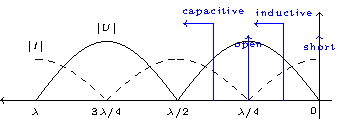
\includegraphics[width=8cm]{Cha3//VolCurDistribution.pdf}\\
  \flushleft
  综上所述,均匀无耗传输线终端无论是短路、开路还是接纯电抗负载,终端均产生全反射,沿线电压电流呈驻波分布,只是终端不同。\\
  1、\textbf{短路}:电压按正弦变化,电流按余弦变化,终端电压为零,电流为最大;\\
  \textbf{开路}:电压按余弦变化,电流按正弦变化,终端电流为零,电压为最大;\\
  \textbf{纯电抗}:电压、电流按正余弦变化,终端电压和电流不为零,也不是最大。
\end{frame}


\begin{frame}{无耗传输线工作状态}
  2、二分之一波长的重复性,四分之一波长的变化性。\\
  3、驻波波腹值为入射波的两倍,波节值等于零。短路线终端为电压波节、电流波腹;开路线终端为电压波腹、电流波节;接纯电抗负载时,终端既非波腹也非波节(\textbf{纯电感负载时,距负载第一个出现的是电压波腹点})。\\
  4、沿线同一位置的电压电流之间$90^\circ$相位差,所以驻波状态只有能量的存贮并无能量的传输。
\end{frame}


\begin{frame}{无耗传输线工作状态}
  \begin{enumerate}
    \resume
    \item \textbf{行驻波状态(部分反射情况)}\quad \fbox{$Z_L=R_L\pm \mathrm{j}X_L$}
  \end{enumerate}
  条件:当均匀无耗传输线终端接一般复阻抗,产生部分反射,在线上形成行驻波。
  \begin{empheq}[box=\widefbox]{align*}
    \Gamma_L & =\frac{Z_L-Z_0}{Z_L+Z_0}=\frac{(R_L\pm \mathrm{j}X_L)-Z_0}{(R_L\pm \mathrm{j}X_L)+Z_0}\\
    & = \frac{R_L^2-Z_0^2+X_L^2}{(R_L+Z_0)^2+X_L^2}\pm \mathrm{j}\frac{2X_LZ_0}{(R_L+Z_0)^2+X_L^2}\\
    & = \Gamma_{L1}\pm \mathrm{j}\Gamma_{L2}=\lvert \Gamma_L\rvert \mathrm{e}^{\pm \mathrm{j}\phi_L}
  \end{empheq}
\end{frame}


\begin{frame}{无耗传输线工作状态}
  \widefbox{$\Gamma_L=\lvert\Gamma_L\rvert \mathrm{e}^{\pm \mathrm{j}\phi_L}$}
  \begin{align*}
     & \lvert\Gamma_L\rvert=\sqrt{\frac{(R_L-Z_0)^2+X_L^2}{(R_L+Z_0)^2+X_L^2}}<1 \\
     & \phi_L=\arctan\frac{\pm 2X_LZ_0}{R_L^2+X_L^2-Z_0^2}
  \end{align*}
  传输线工作在行驻波状态,行波与驻波的相对大小决定于负载与传输线的失配程度。
\end{frame}


\begin{frame}{无耗传输线工作状态}
  1、沿线电压、电流分布\\
  从
  \begin{align*}
    V(d)=V^+(d)[1+\lvert\Gamma_L\rvert \mathrm{e}^{\mathrm{j}(\phi_L-2\beta d)}] \\
    I(d)=I^+(d)[1-\lvert\Gamma_L\rvert \mathrm{e}^{\mathrm{j}(\phi_L-2\beta d)}]
  \end{align*}
  \begin{empheq}[box=\widefbox]{align*}
    V(d)=V_L^+\mathrm{e}^{\mathrm{j}\beta d}[1+\lvert\Gamma_L\rvert \mathrm{e}^{\phi_L-2\beta d}]\\
    I(d)=I_L^+\mathrm{e}^{\mathrm{j}\beta d}[1-\lvert\Gamma_L\rvert \mathrm{e}^{\phi_L-2\beta d}]
  \end{empheq}
  $\xLongrightarrow{\text{取模}}$
  \begin{align*}
     & \lvert V\rvert_{\mathrm{max}}=V_L^+[1+\lvert\Gamma_L\rvert] \qquad \lvert V\rvert_{\mathrm{min}}=V_L^+[1-\lvert\Gamma_L\rvert]      \\
     & \lvert I\rvert_{\mathrm{max}}=I_L^+[1+\lvert\Gamma_L\rvert] \qquad\quad \lvert I\rvert_{\mathrm{min}}=I_L^+[1-\lvert\Gamma_L\rvert]
  \end{align*}
  此时$\lvert\Gamma\rvert<1$,终端产生部分反射,线上形成行驻波,无波节点,驻波最小值不等于零,驻波最大值不等于终端入射波振幅的两倍。
\end{frame}



\begin{frame}{无耗传输线工作状态}
  \begin{align*}
    \lvert V(d)\rvert=\lvert V^+(d)\rvert[1+\lvert\Gamma_L\rvert^2+2\lvert\Gamma_L\rvert\cos(\phi_L-2\beta d)]^{1/2} \\
    \lvert I(d)\rvert=\lvert I^+(d)\rvert[1+\lvert\Gamma_L\rvert^2-2\lvert\Gamma_L\rvert\cos(\phi_L-2\beta d)]^{1/2}
  \end{align*}
  当$\cos(\phi_L-2\beta d)=1$\quad $\Longrightarrow$\quad \widefbox{$\phi_L-2\beta d=-2n\pi$}\\
  电压驻波最大点位置
  \begin{empheq}[box=\widefbox]{align*}
    d_{max}=\frac{\lambda}{4\pi}\phi_L+n\frac{\lambda}{2}\quad n=0,1,2,\ldots
  \end{empheq}
  当$\cos(\phi_L-2\beta d)=-1$\quad $\Longrightarrow$\quad \widefbox{$\phi_L-2\beta d=-\pi-2n\pi$}\\
  电压驻波最小点位置
  \begin{empheq}[box=\widefbox]{align*}
    d_{min}=\frac{\lambda}{4\pi}\phi_L+\frac{\lambda}{4}(2n+1)\quad n=0,1,2,\ldots
  \end{empheq}
\end{frame}



\begin{frame}{无耗传输线工作状态}
  2、阻抗分布
  \begin{align*}
    Z_{in}(d)  =Z_0\frac{1+\lvert\Gamma_L\rvert \mathrm{e}^{-\mathrm{j}(2\beta d-\phi_L)}}{1-\lvert\Gamma_L\rvert \mathrm{e}^{-\mathrm{j}(2\beta d-\phi_L)}}=Z_0\frac{\mathrm{e}^{\mathrm{j}(\beta d-\frac{1}{2}\phi_L)}+\lvert\Gamma_L\rvert \mathrm{e}^{-\mathrm{j}(\beta d-\frac{1}{2}\phi_L)}}{\mathrm{e}^{\mathrm{j}(\beta d-\frac{1}{2}\phi_L)}-\lvert\Gamma_L\rvert \mathrm{e}^{-\mathrm{j}(\beta d-\frac{1}{2}\phi_L)}} \\
    = Z_0\frac{(1+\lvert\Gamma_L\rvert)\cos\left(\beta d-\frac{1}{2}\phi_L\right)+\mathrm{j}(1-\lvert\Gamma_L\rvert)\sin\left(\beta d-\frac{1}{2}\phi_L\right)}{(1-\lvert\Gamma_L\rvert)\cos\left(\beta d-\frac{1}{2}\phi_L\right)+\mathrm{j}(1+\lvert\Gamma_L\rvert)\sin\left(\beta d-\frac{1}{2}\phi_L\right)}
  \end{align*}
  \begin{empheq}[box=\widefbox]{align*}
    Z_{in}(d)=Z_0\frac{\left(\frac{1+\lvert\Gamma_L\rvert}{1-\lvert\Gamma_L\rvert}\right)+\mathrm{j}\tan\left(\beta d-\frac{1}{2}\phi_L\right)}{1+\mathrm{j}\left(\frac{1+\lvert\Gamma_L\rvert}{1-\lvert\Gamma_L\rvert}\right)\tan\left(\beta d-\frac{1}{2}\phi_L\right)}
  \end{empheq}
  \begin{empheq}[box=\widefbox]{align*}
    \rho=\frac{1+\lvert\Gamma_L\rvert}{1-\lvert\Gamma_L\rvert}
  \end{empheq}
\end{frame}



\begin{frame}{无耗传输线工作状态}
  \begin{align*}
     & \cos(\phi_L-2\beta d)=1,\qquad \text{(V最大 I最小)} \\
     & Z_{in}=R_{max}+\mathrm{j}X_{max}=Z_0\rho        \\
     & R_{max}=Z_0\rho;X_{max}=0
  \end{align*}
  \hspace*{\fill}
  \begin{align*}
     & \cos(\phi_L-2\beta d)=-1,\qquad \text{(V最小 I最大)} \\
     & Z_{in}=R_{min}+\mathrm{j}X_{min}=Z_0/\rho        \\
     & R_{min}=Z_0/\rho=Z_0K;X_{min}=0
  \end{align*}
  \hspace*{\fill}
  \begin{align*}
     & \text{电压最大、最小点阻抗均为实数,二者相距}\lambda/4, \\
     & R_{max}R_{min}=Z_{0}^{2}
  \end{align*}
\end{frame}

\subsection{广义无耗传输线求解}


\begin{frame}{广义无耗传输线求解}
  \centering
  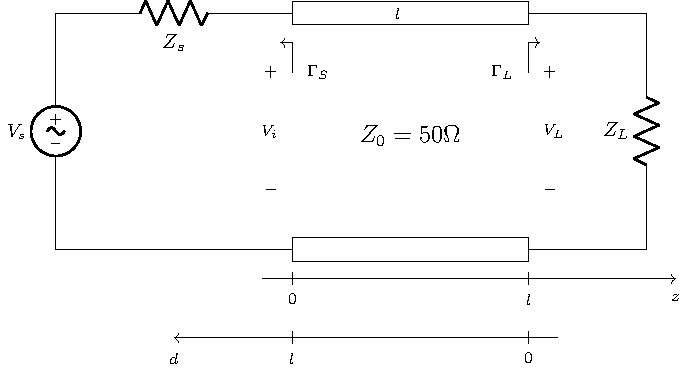
\includegraphics[width=11cm]{Cha3//fig3-16.pdf}
\end{frame}


\begin{frame}{广义无耗传输线求解}

  \flushleft
  边界条件:
  \begin{align}
    z=0\longrightarrow   \notag                                                                                                                                              \\
    V_i       & =V_s-Z_sI_i=V_0^++V_0^- \qquad   I_i =\frac{V_0^+-V_0^-}{Z_0} \notag                                                                                         \\
    z=l\longrightarrow              \notag                                                                                                                                   \\
    V_L       & =Z_LI_L    \qquad      I_L =\frac{1}{Z_0}\left( V_0^+\mathrm{e}^{-\mathrm{j}\beta l}-V_0^-\mathrm{e}^{\mathrm{j}\beta l}\right) \notag                       \\
    0\leqslant z \leqslant l \longrightarrow  \notag                                                                                                                         \\
    V(z)      & = V^+(z)+V^-(z) = V_0^+\mathrm{e}^{-\mathrm{j}\beta z}\left[ 1+\Gamma(z)\right]\label{eqn1}                                                                  \\
    I(z)      & = I^+(z)-I^-(z) = \frac{V_0^+}{Z_0}\mathrm{e}^{-\mathrm{j}\beta z}\left[1-\Gamma(z)\right]\label{eqn2}                                                       \\
    \Gamma(z) & =\dfrac{V^-(z)}{V^+(z)}=\dfrac{V_0^-\mathrm{e}^{\mathrm{j}\beta z}}{V_0^+\mathrm{e}^{-\mathrm{j}\beta z}}=\Gamma_L\mathrm{e}^{-2\mathrm{j}\beta(l-z)} \notag
  \end{align}

\end{frame}

\begin{frame}{广义无耗传输线求解}
  应用$z=0$处的边界条件
  \begin{align}
    V_i & =V(0)=V_S-Z_S\frac{V_0^+ - V_0^-}{Z_0}=V_0^+ + V_0^-                         \\
    V_S & =V_0^+\left( 1+\frac{Z_S}{Z_0}\right) + V_0^-\left( 1-\frac{Z_S}{Z_0}\right)
  \end{align}
  由$\Gamma_S=\dfrac{Z_S-Z_0}{Z_S+Z_0}$得\\
  \begin{align}
    V_0^- & =V_S\frac{Z_0}{Z_0-Z_S}+\frac{V_0^+}{\Gamma_S}\label{eqn5}
  \end{align}

  应用$z=l$处的边界条件
  \begin{align}
     & V_L=Z_LI_L=\frac{Z_L}{Z_0}(V_0^+\mathrm{e}^{-\mathrm{j}\beta l}-V_0^-\mathrm{e}^{\mathrm{j}\beta l})=V_0^+\mathrm{e}^{-\mathrm{j}\beta l}+V_0^-\mathrm{e}^{\mathrm{j}\beta l} \\
     & \rightarrow \quad V_0^+(Z_0-Z_L)\mathrm{e}^{-\mathrm{j}\beta l}+V_0^-(Z_0+Z_L)\mathrm{e}^{\mathrm{j}\beta l}=0\label{eqn7}
  \end{align}
\end{frame}

\begin{frame}{广义无耗传输线求解}
  由式(\ref{eqn5})和式(\ref{eqn7})联立可得
  \begin{align}
    V_0^+ & =V_S\frac{Z_0}{Z_0+Z_S}\cdot\frac{1}{1-\Gamma_S\Gamma_L\mathrm{e}^{-2\mathrm{j}\beta l}}\label{eqn8}
  \end{align}
  式中$\Gamma_L=\dfrac{Z_L-Z_0}{Z_L+Z_0}$\\
  将式(\ref{eqn8})代入式(\ref{eqn1})和(\ref{eqn2}),即可得到一般情况下的$V(z)$和$I(z)$表达式为
  \begin{align}
    V(z) & =\frac{Z_0V_S}{Z_0+Z_S}\mathrm{e}^{-\mathrm{j}\beta z}\left(\frac{1+\Gamma_L\mathrm{e}^{-\mathrm{j}2\beta(l-z)}}{1-\Gamma_S\Gamma_L\mathrm{e}^{-\mathrm{j}2\beta l}}\right)\label{eqn9} \\
    I(z) & =\frac{V_S}{Z_0+Z_S}\mathrm{e}^{-\mathrm{j}\beta z}\left(\frac{1-\Gamma_L\mathrm{e}^{-\mathrm{j}2\beta(l-z)}}{1-\Gamma_S\Gamma_L\mathrm{e}^{-\mathrm{j}2\beta l}}\right)\label{eqn10}
  \end{align}
\end{frame}

\begin{frame}{广义无耗传输线求解}
  根据二项式公式
  \begin{empheq}[box=\widefbox]{align*}
    \color{blue}{(1+x)^n=1+nx+\frac{n(n-1)}{2!}x^2+\ldots}
  \end{empheq}

  \begin{align}
    (1-\Gamma_S\Gamma_L\mathrm{e}^{-\mathrm{j}2\beta l})^{-1} & =1+\Gamma_S\Gamma_L\mathrm{e}^{-\mathrm{j}2\beta l}+\Gamma_S^2\Gamma_L^2\mathrm{e}^{-\mathrm{j}4\beta l}+\ldots \label{eqn11}
  \end{align}

  将式(\ref{eqn11})代入式(\ref{eqn9})和(\ref{eqn10})中得

  \begin{equation}
    \begin{split}
      V(z)&=\frac{V_S}{Z_0+Z_S}\cdot Z_0[\mathrm{e}^{-\mathrm{j}\beta z}+\Gamma_L\mathrm{e}^{-\mathrm{j}\beta(2l-z)}\\
      &+\Gamma_S\Gamma_L\mathrm{e}^{-\mathrm{j}\beta(2l+z)}+\Gamma_S\Gamma_L^2\mathrm{e}^{-\mathrm{j}\beta(4l-z)}+\ldots]\label{eqn12}
    \end{split}
  \end{equation}
  \begin{equation}
    \begin{split}
      I(z)&=\frac{V_S}{Z_0+Z_S}[\mathrm{e}^{-\mathrm{j}\beta z}-\Gamma_L\mathrm{e}^{-\mathrm{j}\beta(2l-z)}\\
      &+\Gamma_S\Gamma_L\mathrm{e}^{-\mathrm{j}\beta(2l+z)}-\Gamma_S\Gamma_L^2\mathrm{e}^{-\mathrm{j}\beta(4l-z)}+\Gamma_S^2\Gamma_L^2\mathrm{e}^{-\mathrm{j}\beta(4l+z)}-\ldots]\label{eqn13}
    \end{split}
  \end{equation}
\end{frame}

\begin{frame}{广义无耗传输线求解}
  式(\ref{eqn12})可展开为
  $$V(z)=V_1^++V_1^-+V_2^++\cdots=\sum_{i=1}^{\infty}(V_i^++V_i^-)$$
  式中
  \begin{align*}
    \lvert V_1^+\rvert & = \left\lvert \left(\frac{Z_0}{Z_0+Z_S}V_S\right)\right\rvert                                           \\
    \lvert V_1^-\rvert & = \lvert\Gamma_L\rvert\left\lvert \left(\frac{Z_0}{Z_0+Z_S}V_S\right)\right\rvert                       \\
    \lvert V_2^+\rvert & = \lvert\Gamma_S\rvert\lvert\Gamma_L\rvert\left\lvert \left(\frac{Z_0}{Z_0+Z_S}V_S\right)\right\rvert   \\
    \lvert V_2^-\rvert & = \lvert\Gamma_S\rvert\lvert\Gamma_L\rvert^2\left\lvert \left(\frac{Z_0}{Z_0+Z_S}V_S\right)\right\rvert
  \end{align*}
\end{frame}

\begin{frame}{广义无耗传输线求解}
  式(\ref{eqn13})可展开为
  $$I(z)=I_1^+-I_1^-+I_2^+-I_2^-+\cdots=\sum_{i=1}^{\infty}(I_i^+-I_i^-)$$
  \begin{align*}
    z=0\text{注入电流}      & \quad I^+(0)=\frac{V_S}{Z_0+Z_S}                                                                                \\
                        & \downarrow                                                                                                      \\
    \text{正行至}z         & \quad I_1^+=\frac{V_S}{Z_0+Z_S}\mathrm{e}^{-\mathrm{j}\beta z}                                                  \\
                        & \downarrow                                                                                                      \\
    \text{正行至终端}        & \quad I^+(l)=\frac{V_S}{Z_0+Z_S}\mathrm{e}^{-\mathrm{j}\beta l}                                                 \\
                        & \downarrow                                                                                                      \\
    \text{经负载反射后,再反行至}z & \quad I_1^-=\mathrm{e}^{-\mathrm{j}\beta (l-z)}=\Gamma_L\frac{V_S}{Z_0+Z_S}\mathrm{e}^{-\mathrm{j}\beta (2l-z)} \\
                        & \downarrow
  \end{align*}
\end{frame}

\begin{frame}{广义无耗传输线求解}
  \begin{columns}
    \begin{column}{0.5\linewidth}
      \begin{center}
        再反行至源端
        \begin{align*}
          I^-(0)= & \Gamma_L\frac{V_S}{Z_0+Z_S}\mathrm{e}^{-\mathrm{j}2\beta l} \\
                  & \downarrow
        \end{align*}
      \end{center}

      \begin{center}
        经源端反射后,再正行到$z$
        \begin{align*}
          I_2^+(0)= \Gamma_S\Gamma_L & \frac{V_S}{Z_0+Z_S}\mathrm{e}^{-\mathrm{j}\beta(2l+z)} \\
                                     & \vdots
        \end{align*}
      \end{center}

    \end{column}
    \begin{column}{0.5\linewidth}
      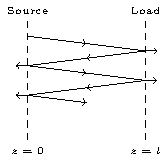
\includegraphics[width=5cm]{Cha3//fig3-17.pdf}
    \end{column}
  \end{columns}

\end{frame}

\begin{frame}{广义无耗传输线求解}{两端均匹配}
  \begin{columns}
    \begin{column}{0.5\linewidth}
      \begin{align*}
         & \color{blue}{Z_S=Z_L=Z_0 \quad \Gamma_S=\Gamma_L=0}                                                          \\
         & V(z)=\frac{V_S}{2}\mathrm{e}^{-\mathrm{j}\beta z} \quad I(z)=\frac{V_S}{2Z_0}\mathrm{e}^{-\mathrm{j}\beta z} \\
         & \text{源端}(z=0)                                                                                               \\
         & V(0)=V_i=\frac{V_S}{2} \quad I(0)=I_i=\frac{V_S}{2Z_0}                                                       \\
      \end{align*}
      \begin{empheq}[box=\widefbox]{align*}
        &|V_0^+|=|V_i|=|V_L|=|V(z)|=\frac{V_S}{2}\\
        &|I_0^+|=|I_i|=|I_L|=|I(z)|=\frac{V_S}{2Z_0}
      \end{empheq}
    \end{column}
    \begin{column}{0.5\linewidth}
      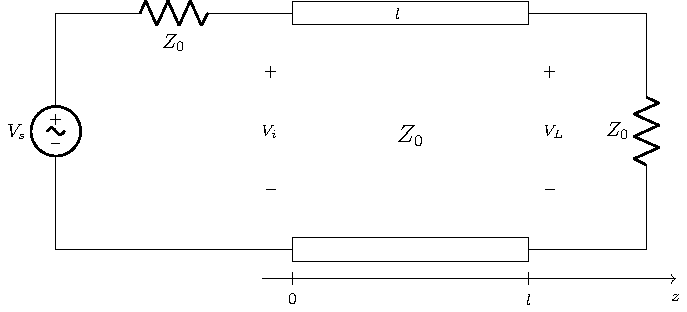
\includegraphics[width=6cm]{Cha3//fig3-18.pdf}
      \begin{align*}
         & \text{负载端}(z=l)                                          \\
         & V(l)=V_L=\frac{V_S}{2}\mathrm{e}^{-\mathrm{j}\beta l}    \\
         & I(l)=I_L=\frac{V_S}{2Z_0}\mathrm{e}^{-\mathrm{j}\beta l}
      \end{align*}
    \end{column}
  \end{columns}
  \flushleft

  传输线上不存在驻波,沿线各处的电压和电流幅度均相等
\end{frame}


\begin{frame}{广义无耗传输线求解}{仅源端匹配}
  \begin{columns}
    \begin{column}{0.5\linewidth}
      \begin{align*}
         & \color{blue}{Z_S=Z_0,Z_L\neq Z_0 \quad \Gamma_S=0,\Gamma_L\neq 0}                                   \\
         & V(z)=\frac{V_S}{2}\mathrm{e}^{-\mathrm{j}\beta z}(1+\Gamma_L\mathrm{e}^{-\mathrm{j}2\beta(l-z)})    \\
         & I(z)=\frac{V_S}{2Z_0}\mathrm{e}^{-\mathrm{j}\beta z}(1-\Gamma_L\mathrm{e}^{-\mathrm{j}2\beta(l-z)}) \\
         & \text{源端}(z=0)                                                                                      \\
         & V(0)=V_i=\frac{V_S}{2}(1+\Gamma_L\mathrm{e}^{-\mathrm{j}2\beta l})                                  \\
         & I(0)=I_i=\frac{V_S}{2Z_0}(1-\Gamma_L\mathrm{e}^{-\mathrm{j}2\beta l})                               \\
         & \text{负载端}(z=l)
      \end{align*}
    \end{column}
    \begin{column}{0.5\linewidth}
      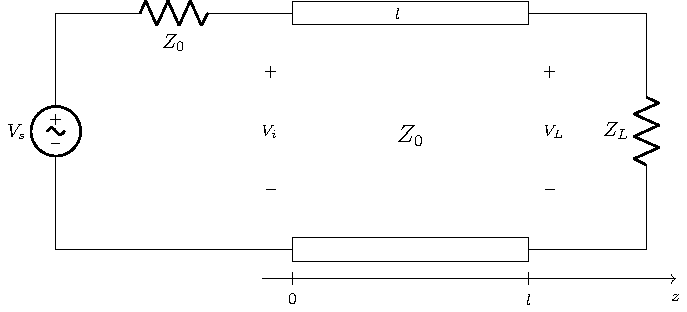
\includegraphics[width=6cm]{Cha3//fig3-19.pdf}
    \end{column}
  \end{columns}
  \flushleft
  $V(l)=V_L=\dfrac{V_S}{2}\mathrm{e}^{-\mathrm{j}\beta l}(1+\Gamma_L)\quad I(l)=I_L=\dfrac{V_S}{2Z_0}\mathrm{e}^{-\mathrm{j}\beta l}(1-\Gamma_L)$
\end{frame}


\begin{frame}{广义无耗传输线求解}{仅负载端匹配}
  \begin{columns}
    \begin{column}{0.5\linewidth}
      \begin{align*}
         & \color{blue}{Z_S\neq Z_0,Z_L=Z_0 \quad \Gamma_S\neq 0,\Gamma_L= 0} \\
         & V(z)=\frac{V_S}{2}\mathrm{e}^{-\mathrm{j}\beta z}\quad
        I(z)=\frac{V_S}{2Z_0}\mathrm{e}^{-\mathrm{j}\beta z}                  \\
         & \text{源端}(z=0)                                                     \\
         & V(0)=V_i=\frac{V_SZ_0}{Z_0+Z_S}                                    \\
         & I(0)=I_i=\frac{V_S}{Z_0+Z_S}                                       \\
         & \text{负载端}(z=l)                                                    \\
         & V(l)=V_L=\frac{Z_0V_S}{Z_0+Z_S}\mathrm{e}^{-\mathrm{j}\beta l}     \\
         & I(l)=I_L=\frac{V_S}{Z_0+Z_S}\mathrm{e}^{-\mathrm{j}\beta l}
      \end{align*}
    \end{column}
    \begin{column}{0.5\linewidth}
      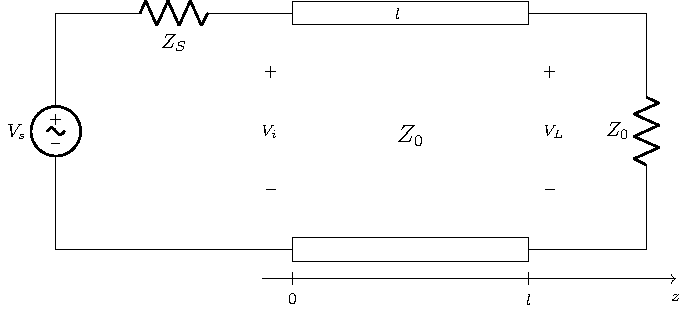
\includegraphics[width=6cm]{Cha3//fig3-20.pdf}
      \begin{empheq}[box=\widefbox]{align*}
        &V_i=V_L\mathrm{e}^{\mathrm{j}\beta l}\\
        &V(z)=V_L\mathrm{e}^{-\mathrm{j}\beta(z-l)}\\
        &I_i=I_L\mathrm{e}^{\mathrm{j}\beta l}\\
        &I(z)=I_L\mathrm{e}^{-\mathrm{j}\beta(z-l)}
      \end{empheq}
      沿线各处的电压和电流\textbf{相位}随线长而变化,\textbf{幅度}不变。
    \end{column}
  \end{columns}
\end{frame}
